
\documentclass[preprint, 12pt]{elsarticle}


\usepackage[table]{xcolor}
\usepackage{lmodern}

\usepackage[utf8]{inputenc}
\usepackage[T1]{fontenc}
\usepackage{url}

\usepackage{xspace}
\newcommand{\ie}[0]{{\em i.e.},\xspace}
\newcommand{\vs}[0]{{\em vs.}\xspace}
\newcommand{\eg}[0]{{\em e.g.},\xspace}
\newcommand{\etal}[0]{{\em et al.}\xspace}
\newcommand{\wrt}[0]{{\em w.r.t.}\xspace}
\newcommand{\aka}[0]{{\em a.k.a.}\xspace}
\newcommand{\via}[0]{{\em via}\xspace}

\newcommand{\ecotype}[0]{\emph{nantes-ecotype}\xspace}
\newcommand{\nova}[0]{\emph{lyon-nova}\xspace}

\newcommand{\ansass}[0]{\emph{spmd-$1$t}\xspace}
\newcommand{\aeoass}[0]{\emph{dag-$2$t}\xspace}
\newcommand{\madass}[0]{\emph{dag-nt}\xspace}

\newcommand{\shell}[0]{\textsc{Shell}\xspace}
\newcommand{\bash}[0]{\emph{bash}\xspace}
\newcommand{\ansible}[0]{\textsc{Ansible}\xspace}
\newcommand{\chef}[0]{\textsc{Chef}\xspace}
\newcommand{\puppet}[0]{\textsc{Puppet}\xspace}
\newcommand{\cfengine}[0]{\textsc{CFEngine}\xspace}
\newcommand{\deployware}[0]{\textsc{DeployWare}\xspace}
\newcommand{\juju}[0]{\textsc{Juju}\xspace}
\newcommand{\kubernetes}[0]{\textsc{Kubernetes}\xspace}
\newcommand{\aeolus}[0]{\textsc{Aeolus}\xspace}
\newcommand{\mad}[0]{\textsc{Madeus}\xspace}

\newcommand{\kolla}[0]{Kolla\xspace}

\newcommand{\apache}[0]{\textsc{Apache}\xspace}
\newcommand{\mysql}[0]{\textsc{MySQL}\xspace}

\newcommand{\implem}[0]{PoC\xspace}
\newcommand{\llc}{L\textsuperscript{2}C\xspace}
\newcommand{\net}[0]{\emph{internal-net}\xspace}

\usepackage{caption}

\usepackage[colorlinks]{hyperref}
\usepackage{url}

\usepackage[textwidth=17mm]{todonotes}
\newcommand{\customtodo}[4]{
        \todo[color=#2,inline,size=\small]{
                \ifx&#3&
                        \textbf{#1} #4
                \else
                        \textbf{#1$\Rightarrow$#3} #4
                \fi
        }
}
\newcommand{\MC}[2][]{\customtodo{MC}{red!50}{#1}{#2}}
\newcommand{\HC}[2][]{\customtodo{HC}{red!20}{#1}{#2}}
\newcommand{\CP}[2][]{\customtodo{CP}{blue!20}{#1}{#2}}
\newcommand{\DP}[2][]{\customtodo{DP}{blue!50}{#1}{#2}}
\newcommand{\CS}[2][]{\customtodo{CS}{green!20}{#1}{#2}}
\usepackage{amsmath,amssymb,amsfonts}
\usepackage{mathtools}
\usepackage{subfig}
\usepackage{pifont}
\usepackage{wasysym}

\usepackage{booktabs} % For formal tables
\usepackage{array,multirow}
\newcommand{\STAB}[1]{\begin{tabular}{@{}c@{}}#1\end{tabular}}

\usepackage{siunitx}
\usepackage{cleveref}

\usepackage{tikz}
\usetikzlibrary{shapes.geometric, arrows}
\tikzstyle{place} = [rectangle, rounded corners, minimum width=2cm, minimum height=1cm,text centered, draw=black, fill=red!40]
\tikzstyle{leaving} = [rectangle, rounded corners, minimum width=2cm, minimum height=1cm,text centered, draw=black, fill=red!20]
\tikzstyle{provide_start} = [rectangle, rounded corners, minimum width=2cm, minimum height=1cm,text centered, draw=black, fill=orange!40]
\tikzstyle{provide_stop} = [rectangle, rounded corners, minimum width=2cm, minimum height=1cm,text centered, draw=black, fill=blue!20]
\tikzstyle{use_start} = [rectangle, rounded corners, minimum width=2cm, minimum height=1cm,text centered, draw=black, fill=orange!20]
\tikzstyle{use_stop} = [rectangle, rounded corners, minimum width=2cm, minimum height=1cm,text centered, draw=black, fill=blue!40]
\tikzstyle{end} = [rectangle, rounded corners, minimum width=2cm, minimum height=1cm,text centered, draw=black, fill=gray!20]
\tikzstyle{beginning} = [rectangle, rounded corners, minimum width=2cm, minimum height=1cm,text centered, draw=black, fill=gray!40]
\tikzstyle{control} = [rectangle, rounded corners, minimum width=2cm, minimum height=1cm,text centered, draw=black, fill=orange!30]
\tikzstyle{arrow} = [thick,->,>=stealth]

\def\cmark{\tikz\fill[scale=0.4](0,.35) -- (.25,0) -- (1,.7) -- (.25,.15) -- cycle;}

% lstlisting python + colors
\usepackage{color}
\usepackage[procnames]{listings}
\definecolor{keywords}{RGB}{255,0,90}
\definecolor{comments}{RGB}{0,0,113}
\definecolor{red}{RGB}{160,0,0}
\definecolor{green}{RGB}{0,150,0}
\definecolor{backcolour}{rgb}{0.95,0.95,0.95}
\DeclareCaptionFont{white}{\color{white}}
\DeclareCaptionFormat{listing}{\colorbox{gray}{\parbox{\linewidth}{#1#2#3}}}
\captionsetup[lstlisting]{format=listing,labelfont=white,textfont=white}
\lstset{language=Python,
        numbers=left,
        backgroundcolor=\color{backcolour},
        numbersep=5pt,
        keywordstyle=\color{keywords},
        commentstyle=\color{comments},
        stringstyle=\color{red},
        showstringspaces=false,
        identifierstyle=\color{green},
        procnamekeys={def,class},
        basicstyle=\scriptsize\ttfamily,
        numberstyle=\tiny\color{gray},
%       frame=single
}

% Fix for bibliography
\makeatletter
\providecommand{\doi}[1]{%
  \begingroup
    \let\bibinfo\@secondoftwo
    \urlstyle{rm}%
    \href{http://dx.doi.org/#1}{%
      doi:\discretionary{}{}{}%
      \nolinkurl{#1}%
    }%
  \endgroup
}
\makeatother


\journal{Journal of Systems and Software}

\begin{document}

\begin{frontmatter}

\title{Madeus}

\author[label1]{Maverick Chardet}
\ead{maverick.chardet@inria.fr}
\author[label1]{Hélène Coullon}
\author[label1]{Dimitri Pertin}
\author[label1]{Charlène Servantie}
%\ead{\{maverick.chardet, helene.coullon, christian.perez, \
%       dimitri.pertin, charlene.servantie\}@inria.fr}
\address[label1]{IMT Atlantique, Inria, LS2N, UBL, F-44307 Nantes, France}

\author[label2]{Christian Perez}
\address[label2]{Univ. Lyon, Inria, CNRS, ENS de Lyon, UCBL 1, LIP, Lyon, France}


\begin{abstract}
\end{abstract}

\begin{keyword}
Science \sep Publication \sep Complicated
\end{keyword}

\end{frontmatter}


%-------------------------------------------------------
\section{Introduction}
\label{sec:introduction}
%-------------------------------------------------------
%This paper focuses on one specific challenge related to distributed
%software deployment: \emph{distributed software commissioning}. By
%software commissioning we mean the complete installation,
%configuration and testing process when deploying distributed software
%on physical distributed resources, with or without a virtualization
%layer in between. This process is complex and error-prone because of
%the specificity of the installation process according to the operating
%system, the different kinds of virtualization layers used between the
%physical machines and the pieces of software, the amount of possible
%configuration options~\cite{Xu:2015:SAT:2775083.2791577}. Recently,
%commissioning (or configuration) management tools such as
%Ansible\footnote{\url{https://www.ansible.com/}}, or
%Puppet\footnote{\url{https://puppet.com}}, have been widely adopted by
%system operators. These tools commonly include good
%software-engineering practices such as code reuse and composition in
%management and configuration scripts. It is nowadays possible to build
%a new installation by assembling different pieces of existing
%installations\footnote{\url{https://galaxy.ansible.com/}}\footnote{\url{https://forge.puppet.com/}}
%which improves the productivity of system operators and prevents many
%errors. Many distributed software commissioning are nowadays written
%with one the three above tools and by using containers between the
%host operating system and the pieces of software, such that
%portability of installations is improved. For instance, OpenStack,
%which is the de-facto open source operating system of Cloud
%infrastructures, can be automatically installed on clusters by using
%the
%\href{https://docs.openstack.org/kolla-ansible/latest/}{\emph{kolla-ansible}
%  project}, which uses both Docker containers and Ansible.
%
%Yet, even for such well-established software, there is still much room
%for improving the efficiency of the commissioning process (\ie
%reducing deployment times, minimizing services interruptions etc.).


In contrast to monolithic software that runs locally on a single machine, distributed software is designed in a modular architectural style where each entity (\ie module, component, or service or micro-service) is responsible for a specific part of the overall objective, and collaborates at runtime with other entities that are potentially hosted on distant nodes (\ie machines). In the rest of this paper we will use the generic term \emph{component} to refer indifferently to a module, a service or a micro-service. Distributed software have become commonplace in our day-to-day life, sometimes hosted on the Cloud, on personal computers, on mobile phones, on objects etc. 

However, deploying a large distributed software on infrastructures is a tedious task where components have to be chosen and mapped to the nodes of infrastructures, where components have to be chosen and configured, where dependencies have to be solved, where virtualization layers have to be handled etc. Furthermore, such procedure involves many different actors with different expertise and roles which increase the difficulty of the overall process: (1) \emph{developers} who are responsible for designing and coding a set of components or services; (2) \emph{sysadmins} and \emph{sysops} responsible for up-keeping, configuring, and testing multi-users computer systems such as servers or Clouds, and (3) in between \emph{devops} engineers that work with software developers, system operators (SysOps) and other production IT staff to oversee code releases and deployments. For these reasons, deployment procedures have to be automated and need adapted programming support (\ie languages, models).

In this paper, among the difficulties related to the deployment of distributed software systems, we left apart the mapping between pieces of software and the nodes of the infrastructure, which is the result of an optimization problem and not in the scope of this paper~\cite{6409358, 10.1007/978-3-319-47677-3_15, cadorel:hal-02165835, ccgridemile, 10.5555/2432523.2432528}. Indeed, we restrict the scope of this paper to the \emph{software-commissioning} part of the deployment, \ie the procedure responsible for leading the set of components to a valid running state while guaranteeing correct configurations and interactions.
%
In particular, three metrics are considered important regarding the quality of
the automation of distributed software commissioning in this paper: (1) a clear separation of concerns between the different actors of the commissioning procedure (\ie developers, sysadmins and devops) to enhance productivity, maintainability
and re-usability of deployment codes; (2) the efficiency of the commissioning procedure in terms of parallelism expressiveness; and (3) the formalization of the solution such that formal properties can be proven on a given commissioning procedure. The contribution of this paper improves the related work by succeeding in the combination of these three metrics.
%

In~\cite{chardet:hal-01858150} we have presented a formal model for distributed software commissioning, namely \mad, that theoretically improves the parallelism
level exposed to the user. This journal paper brings the following additional
contributions compared to our previous publication: 
\begin{itemize} 
	\item an extended study of the related work; 
	\item a revised and streamlined \mad formal	model that offers stronger guarantees; 
	\item a theoretical performance prediction model of \mad; 
	\item a concrete language and a prototype;
	\item an extended reproducible evaluation on both synthetic use-cases and one large real use-case on real infrastructures.
\end{itemize}

%%% outline
The rest of this paper is organized as follows. Section~\ref{sec:motivation} presents the detailed motivations of the contribution. Section~\ref{sec:related_work} studies the related work. Section~\ref{sec:mad_model} gives an overview of \mad as well as its concrete language. Sections~\ref{sec:formal_model} and~\ref{sec:perf_model} respectively detail the formalization of \mad as well as its associated performance prediction model. Sections~\ref{sec:evaluations} and~\ref{sec:use-cases} respectively present an evaluation of the \mad prototype on synthetic use-cases and an evaluation of the contribution interests on the real use-case of OpenStack commissioning.  Finally, Section~\ref{sec:conc} concludes and gives some perspectives.






%-------------------------------------------------------
\section{Related Work}
\label{sec:related_work}
%-------------------------------------------------------
% 1. introduce metrics of RW
% - soft. eng., composition, code reuse, sep of concerns
% - parallelism levels
% 2. RW analyze
% - each tool
% - table
% 3. discussion
% - intra-task
% - performance model

%----------------------------
\subsection{Related work metrics}
%----------------------------
% 1. software engineering
% - components / service / module
% - sub-elements / tasks
% - separation of concerns when assembling 2 components, no need to
% know what each component does to commission itself
% 2. parallelism
% - node / SIMH
% - inter-component
% - inter-task
% - intra-task
% 3. formalism
% - formal model

Before introducing the related work of this paper, some analysis
metrics need to be introduced. These metrics are divided in three
sets: software engineering (SE) metrics, metrics related to the
parallelism level of commissionings, and metrics related to formal
aspects of commissionings. For each metric four levels will be
considered and presented in Table~\ref{tab:comparison}: (1) supported,
denoted with \checkmark, that counts for 3 points in the score; (2)
partially supported, denoted (\checkmark), that counts for 2 points;
(3) manually supported, denoted \emph{M}, meaning that the user may
code manually the given metric, and that counts 1 point; and finally
(4) not supported, denoted -.

\paragraph{Software engineering}
As introduced in the previous section, when automating distributed
software commissionings one important aspect is to promote software
engineering properties. Indeed, when different actors are involved in
a same given goal, software engineering techniques can help improving
separation of concerns (\ie code reuse, maintainability
etc.). Separation of concerns means that each actor is responsible for
her own specialism, \ie her own expertise domain. Such separation of
concerns is improved as soon as a modular or component-based approach
is adopted, \ie each actor could be responsible for one
component. Furthermore, component-based architectures are also equiped
with composition mechanisms that ease the interactions between the
different entities implemented by different actors. One additional
actor may also enter the picture to design this composition. We define
three SE metrics to compare the related work:
\begin{itemize}
\item \emph{component}: if the work (tool, framework or scientific
  contribution) offers a component-oriented (\eg services, modules)
  structure of commissionings;
\item \emph{tasks}: if the work (tool, framework or scientific
  contribution) offers a way to divide the commissioning of each
  component in sub-elements that we call \emph{tasks} and that promote
  even more a well structured procedural design;
\item \emph{separation of concerns}: if the work (tool, framework or
  scientific contribution) offers a way to build distributed software
  commissionings by composing each commissioning of individual
  components and while not needing to know their internal behaviors.
\end{itemize}

\paragraph{Parallelism level}
A second important aspect of distributed software commissioning that
has been introduced in the previous section is its efficiency and in
particular (in this paper) the level of parallelism offered by
commissioning tools and frameworks. We consider four metrics to
compare the related work:
\begin{itemize}
\item \emph{SIMH}: if the work offers a transparent way to perform the
  same instruction or set of instructions on multiple hosts
  simultaneously, meaning that there are no dependencies between the
  instructions to perform on the different hosts;
  \item \emph{inter-comp}: if the work offers a transparent way to
    simultaneously execute the commissionings of multiple components
    if no dependency exists between those components;
  \item \emph{inter-comp-tasks}: if the work offers a transparent way to
    simultaneously execute the commissioning tasks of multiple
    components until a dependency between multiple tasks is reached;
  \item \emph{intra-comp-tasks}: if the work offers a way to simultaneously
    execute two commissioning tasks of a given component, in other
    words if a partial order of tasks can be given for a component.
\end{itemize}
One can note that the level of parallelism offered by a given tool is
directly correlated to the type of dependencies that can be declared
by users. For instance, without any dependency mechanisms the best
possible level would be SIMH, while with inter-components dependencies
or \emph{inter-comp-tasks} dependencies more parallelism can be
handled between components of different types.

\HC[Helene]{Add figures to explain the four parallelism levels}

One can note that presented metrics for both SE and parallelism are
procedural-oriented as they consider \emph{tasks} and not
\emph{resources}, thus excluding \puppet or \salt for instance. While
being an approach with great advantages, declarative approaches are
not considered in this paper.

\paragraph{Formalism}
The last metric considered to compare the related work is the
existence of a formal model for each commissioning solution. Indeed,
we claim that studying formally commissioning models and their
operational semantics is of high importance to open the door to
verification and safety in commissionings and by extension
reconfigurations. For instance, even if this contribution is not
presented in this paper, the formal model \mad has been
successfully used to verify safety properties on distributed software
commissionings by model checking~\cite{coullon:hal-02323641}.

%----------------------------
\subsection{Description and comparison of the related work}
% ----------------------------

Among the plethora of distributed software commissioning solutions, we
have selected a subpart of them for a deeper comparison. According to
the classification of Section~\ref{sec:context}, we have selected: two
\emph{coding} or scripting solutions, \shell and \fractal; three
procedural-oriented solutions of the \emph{software configuration}
class, \ansible, \deployware and \aeolus; two solutions of the
\emph{infrastructure definition} class, \juju and \tosca; and finally
one \emph{orchestration} solution, \kubernetes. In this selection we
have taken a particular attention to select both production tools and
academic contributions. Moreover, we have selected production tools
having a significant opensource community.

% Shell-scripts
\paragraph{Shell scripts}
The traditional way operators automate software commissioning is by
transcribing the actions and configurations from READMEs and tutorials
into a sequence of commands in \shell scripts. On the one hand, those
scripts are written with low-level imperative languages, and with good
programming skills, it is possible to express complex workflows (\eg
idempotency, parallelism, remote actions using \textsc{SSH}). For
instance, parallelism can be managed by combining command execution in
the background (\eg using the control operator \& in \bash) and
synchronisation commands like \emph{wait}. On the other hand, as the
system grows, any custom script becomes error-prone, unpredictable,
hard to understand and to maintain. \shell scripts lack of software
engineering aspects and there is no framework to express modules nor
tasks and their dependencies thus making separation of concerns a very
tricky work. In Table~\ref{tab:comparison} we indicate that each
metric introduced could potentially be implemented manually by using
\shell. Of course, such mechanisms are difficult to implement, error
prone, and time consuming.
% devstack is a set of shell script to deploy OpenStack on a single machine

\paragraph{Fractal}
Component-based software engineering (CBSE) is a domain that enhances
(distributed) software implementation by dealing with code re-use,
separations of concerns, and composability (thus maintainability) of
software codes~\cite{Szyperski:2002:CSB:515228}. A component-based
application is composed of a set of component instances connected
together. Such composition of components is called an
\emph{assembly}. A component is a black box that implements an
independent functionality of an application, and which interacts with
other components through well defined interfaces, called \emph{ports}.
Ports are used to decouple the component internals from its
interface. For instance, a port can be used to declare that the
component either provides a service ---in this case the port is
attached to an internal method--- or use a service from another
component. Many component models focus on the implementation of the
functionalities and
interfaces~\cite{corba:omg06,Blair2009,baude:hal-01001043,Bernholdt01052006,bigot:inria-00388508,Coullon2017}
of components, rather than on their commissioning. A few component
models have contributed to commissioning issues. In the Object
Management Group's (OMG) specification~\cite{ccmdeploy:omg06}, the
commissioning model is rigid and fixed by the model. In
\fractal~\cite{Blair2009} and its evolutions GCM and
GCM/ProActive~\cite{baude:hal-01001043}, the control of a component
(\eg its commissioning) is decoupled from its functionalities into a
so called \emph{membrane} which is itself described as a component
assembly written in java. The membrane is handled by the \fractal
runtime but the sub-assembly and its associated codes are entirely
left to the user. That is why in Table~\ref{tab:comparison}, metrics
not natively supported by \fractal can be handled manually using
java. Both \emph{sparation of concerns} and \emph{inter-comp} are well
handled by \fractal thanks to the notion of port (dependencies within
the component or with an external component) adapted to the
membrane. One can note that only \fractal components commissionings
can be written in the membrane, thus if writing the commissioning of
existing modules they have to be encapsulated in a \fractal component.

% Deployware
\paragraph{Deployware}
\citeauthor{flissi2008ccgrid} proposed \deployware (DW) as a research
effort to distributed software commissioning in the context of Grid
computing~\cite{flissi2008ccgrid}. Its implementation is based on the
\fractal component model. A component is called a \emph{Personality}
and is associated to a fixed set of commissioning actions (\ie
install, configure, start, manage, stop, unconfigure and uninstall),
which can be considered as a fix set of \emph{tasks}.  Each action
describes a sequence of tasks, written with a specific high-level
language that uses pre-defined instructions (\eg execute command, copy
a file). While there is no notion of component ports, it is possible
to express dependencies between components to initiate automatic
coordination. For instance, when the operator triggers the action
"install" on a component, the same action is triggered recursively to
its dependencies. As theyr are not entirely controllable by the user,
metrics \emph{tasks}, \emph{SIMH} and \emph{inter-comp} are considered
as partially supported by \deployware. Finally, as \deployware is
based on \fractal and as a formal effort have been done on \fractal,
the formal aspect of \deployware is considered partially supported.

% Ansible
\paragraph{Ansible}
For the DevOps that are used to shell-scripts, \ansible has become a
popular configuration management tool since it relies on a simple
syntax written in YAML and does not require agents on administrated
servers. Tasks are indeed managed using only \textsc{SSH} and
\textsc{Python} which are commonly installed on every Linux
distributions.  In comparison, similar tools like \chef, \puppet or
\cfengine not only require at least a slight understanding of Ruby or
a custom language to get started, but they are built on an agent-based
architecture and requires prior agent commissioning on remote hosts.
\ansible features software engineering aspects like separation of
concerns by defining the notion of \emph{roles} which can be seen as
software components.  Each role contains a set of files that describe
a sequence of tasks. To define a composition, a specific file called
an \ansible \emph{playbook} is used for mapping the desired roles to
the groups of nodes they will be applied to. Those groups of nodes are
defined in a separate file called the \emph{inventory}. When \ansible
is triggered, roles and their related tasks are sequentially executed
to the associated groups of nodes. While tasks declarations are indeed
manages sequentially, each task is executed in parallel when mapped to
multiple remote hosts thus leading to the \emph{SIMH} metric.
Typically, an operator who wants to commission an \apache web server
and a \mysql database would download two roles from Ansible Galaxy and
register them in an playbook. Since \ansible triggers roles in a
sequential manner, if the operator is not aware that the database must
be commissioned before the web server, she could make a mistake in the
order of the roles she declared. This aspect makes the
\emph{separation of concerns} metric only partially
supported. Finally, as one of the possible type of tasks in \ansible
is the execution of a \shell command, any script could be executed as
a task thus making possible to handle manually the \emph{intra-comp-tasks}
parallelism level.

% Tasks are declared in an imperative way, however, Ansible relies heavily on
% declarative modules, most of which ensure task idempotency (operations are run
% once even if called multiple times).

% Aeolus
\paragraph{Aeolus}
\citeauthor{dicosmo2014ic} proposed \aeolus: a formal component-based
model for the cloud~\cite{dicosmo2014ic}. Their component model
captures the internal states of a component commissioning process
thanks to a finite state machine. Each state can be connected to use,
provide, or conflict ports to declare dependencies between the
commissioning steps of different components. Hence, such ports enable
the coordination of the global deployment process.

% Juju
\paragraph{Juju}
Canonical has developed their own software commissioning solution:
\juju (\url{https://jujucharms.com/}) which aims at commissioning any
kind of application on top of different cloud providers (\eg AWS,
OpenStack), and on multiple types of resources (container, VM or
bare-metal). Its concepts are close to component models. Software
modules are packaged as \juju \emph{charms} which describe the
software commissioning steps through a set of scripts called
\emph{hooks}. Operators define their composition in a specific file
called \emph{bundle} in which they declare the desired charms with
their \emph{relations}. A relation is an element declared between two
charms and used for component synchronization (by triggering hooks)
and data sharing at runtime, similarly to component ports. As the
concepts behind \juju are very close to the one of \aeolus the same
metrics are available except the formal aspect.
% good soc, download charms and run juju deploy

\paragraph{TOSCA}
The \emph{Topology and Orchestration Specification for Cloud
  Applications} (TOSCA) is another component-oriented model that
partially addresses the commissioning of its
components. TOSCA~\cite{tosca:web,10.1007/978-3-319-74781-1_33} is a
standardization effort from OASIS to describe Cloud applications,
their components and their deployment artifacts, using standard
languages (\ie XML, YAML). A TOSCA description (or template)
corresponds to a graph where nodes represent TOSCA resources
(e.g. software components, virtual machines, physical servers), and
where edges represent the relations between those nodes. Artifacts (of
any type: scripts, executable etc.) can be added to TOSCA descriptions
in a CSAR (Cloud Service ARchive) to detail commissioning steps. Those
commissioning steps can thus be customized by the developper but there
is no model and guarantees associated to them. Thus \emph{tasks} and
\emph{intra-comp-tasks} metrics could handled manually by the user. As
there is no way to declare dependencies between artifacts of
components the \emph{inter-taks} metric is not supported, however,
relations between components make both \emph{SIMH} and
\emph{inter-comp} metrics theoretically available in \tosca. No
information have been found on the complete support of these metrics
in \tosca implementations~\cite{cloudify:web,opentosca:web}. Finally,
come efforst have been done to formally define the \tosca
standard~\cite{tosca:web}.

% Kubernetes
\paragraph{Kubernetes}
Initiated by Google, \kubernetes (K8S) is a popular framework to
commission distributed software in the form of micro-services that are
packaged as a hierarchy of Docker containers and \emph{pods}. A
software component in \kubernetes is thus defined as Docker
container. Such components have no port to manage coordination, and
its internals is fixed since containers can only be started and
stopped. As a consequence, the commissioning process is
error-prone. For instance, a web server can be started before the
required database and thus fails. For this reason, the metric
\emph{inter-comp} is considered as partially supported.
% depend_on exists but limited to "container is started"
% synchronization is possible but must be managed by internal script and not managed by k8s
% good soc, download containers and run k8s deploy but without synchonization,
    % commissioning is error-prone

\begin{table*}[tp]
  \centering
  \small
  

% \begin{tabular}{cl|cccccc}
%     \toprule
%     & & Shell & Ansible & DW & K8S & Juju & Aeolus \\
%     \midrule
%     %\rowcolor{gray!15}
%     \multirow{3}{*}{\STAB{\rotatebox[origin=c]{90}{Parallel}}}
%     & node    & \checkmark & \checkmark & \checkmark & \checkmark & \checkmark & \checkmark \\
%     & inter   & \checkmark &   &   &   & \checkmark & \checkmark \\
%     %\rowcolor{gray!15}
%     & intra   & \checkmark &   &   &   &   &   \\
%     \midrule
%     \multirow{2}{*}{\STAB{\rotatebox[origin=c]{90}{SE}}}
%     & module  &   & \checkmark & \checkmark & \checkmark & \checkmark & \checkmark \\
%     %\rowcolor{gray!15}
%     & ports   &   &   &   &   & \checkmark & \checkmark \\
%     \bottomrule
% \end{tabular}

% \newcolumntype{g}{>{\columncolor{gray!15}}c}
% \begin{tabular}{cl|gc|gcgc|gc|g}
%   \toprule
%   \rowcolor{white}
%   & & \multicolumn{2}{c|}{\textit{Coding}} & \multicolumn{4}{c|}{\textit{Software configuration}} & \multicolumn{2}{c|}{\textit{Provisioning}} & \textit{Orchestration} \\
%   \midrule
%   & & \shell & \fractal & \textbf{\ansible} & \puppet & \deployware & \textbf{\aeolus} & \juju & \tosca & \kubernetes \\
%   & & & \cite{} & \cite{} & \cite{} & \cite{} & \cite{} & \cite{} & \cite{} & \cite{} \\ 
%   \midrule
%   \multirow{4}{*}{\STAB{\rotatebox[origin=c]{90}{Soft. eng.}}}
%   & components & M & \checkmark & \checkmark & \checkmark & \checkmark & \checkmark & \checkmark & \checkmark & \checkmark \\
%   & tasks & M & M & \checkmark & M & (\checkmark) & \checkmark & \checkmark & M & \\
%   & resources & M & M & & \checkmark & & & & \checkmark & \\
%   & sep. of con. & M & (\checkmark) & (\checkmark) & \checkmark & \checkmark & (\checkmark) & (\checkmark) & \checkmark & \checkmark \\
%   \midrule
%   \multirow{5}{*}{\STAB{\rotatebox[origin=c]{90}{Parallelism}}}
%   & SIMH & M & (\checkmark) & \checkmark & \checkmark & (\checkmark) & \checkmark & \checkmark & (\checkmark)& \checkmark\\
%   & inter-comp & M & (\checkmark) & & & (\checkmark) & \checkmark & \checkmark & (\checkmark)& (\checkmark)\\
%   & inter-task & M & M & & & & \checkmark & \checkmark & & \\
%   & inter-resource & M & M & & (\checkmark) & & & & (\checkmark) & \\
%   & intra-task & M & M & M & M & M & M & M & M & \\
%   \midrule
%   & formal & & \checkmark & & & (\checkmark) & \checkmark & & \checkmark & \\
%   \midrule
%   & score & 9 & 17 & 11 & 14 & 14 & 20 & 17 & 18 & 11\\
%     \bottomrule
% \end{tabular}

% without resources and puppet

\newcolumntype{g}{>{\columncolor{gray!15}}c}
\begin{tabular}{cl|gc|gcg|cg|c}
  \toprule
  \rowcolor{white}
  & & \multicolumn{2}{c|}{\textit{Coding}} & \multicolumn{3}{c|}{\textit{Software configuration}} & \multicolumn{2}{c|}{\textit{Infrastructure}} & \textit{Orchestration} \\
  \midrule
  & & \shell & \fractal & \deployware & \ansible & \aeolus & \juju & \tosca & \kubernetes \\
  & & & \cite{} & \cite{} & \cite{} & \cite{} & \cite{} & \cite{} & \cite{} \\ 
  \midrule
  \multirow{3}{*}{\STAB{\rotatebox[origin=c]{90}{SE}}}
  & components & M & \checkmark & \checkmark & \checkmark & \checkmark & \checkmark & \checkmark & \checkmark \\
  & tasks & M & M & (\checkmark) & \checkmark & \checkmark & (\checkmark) & M & - \\
  & sep. of con. & M & \checkmark & \checkmark & (\checkmark) & (\checkmark) & (\checkmark) & \checkmark & \checkmark \\
  \midrule
  \multirow{4}{*}{\STAB{\rotatebox[origin=c]{90}{Parallel}}}
  & SIMH & M & \checkmark & (\checkmark) & \checkmark & \checkmark & \checkmark & (\checkmark)& \checkmark\\
  & inter-comp & M & \checkmark & (\checkmark) & - & \checkmark & \checkmark & (\checkmark)& (\checkmark)\\
  & inter-comp-tasks & M & M & - & - & \checkmark & (\checkmark) & - & - \\
  & intra-comp-tasks & M & M & M & M & M & M & M & - \\
  \midrule
  & formal & - & \checkmark & (\checkmark) & - & \checkmark & - & \checkmark & -\\
  \midrule
  & score & 7 & 18 & 15 & 12 & 21 & 16 & 15 & 11\\
    \bottomrule
\end{tabular}



  \caption{Comparison of commissioning solutions based on aspects
  regarding parallelism (performance) and software engineering (SE).}
  \label{tab:comparison}
\end{table*}

%----------------------------
\subsection{Discussions}
%----------------------------
% 3. discussion
% - flexibility vs automation vs formal
% - separation of concerns
% - intra-task parallelism
% - performance model and formal

In the previous section, eight different related works have been
compared according to software engineering metrics, parallelism
metrics and one metric regarding the formal definition of the
considered solution. Table~\ref{tab:comparison} resumes this
comparison and raises a few key points that we discuss in the
following.

As usual when working on programming languages, the existing
tools illustrate the difficult trade-off between flexibility and
automation. On the one hand, when the tool is highly programmable,
developers have the ability to manage their own code organization and
to handle any kind of software engineering or efficiency property. For
instance, by using \shell, any of the introduced metrics could be
handled. However, each of them would have to be hand-coded which is
difficult and error prone. On the other hand, some existing solutions
such as \deployware and \juju restrict the internal commissioning
behavior of components to a fix set of actions (\eg install,
configure, start). Such choice has the advantage of guaranteeing the
full control of the automated parallelism level but also restrict
potential optimizations due to the specificity of each component and
the interactions between components and their tasks.

One can note that \aeolus is the solution with the highest score
regarding the introduced metrics. Indeed, \aeolus combines advantages
of component models to structure the code of software commissionings
and enhance its separation of concerns, while introducing an
additional way to model the internal commissioning behavior of each
component through tasks. It seems that \aeolus offers a good trade-off
between flexibility and automation. However, while offering the best
combination of metrics, \aeolus partially handle separation of
concerns between components.

Furthermore, one can note that no existing solution offers a full
support for \emph{intra-comp-tasks} parallelism level. Actually, if a few
existing solutions already offer a way to model the internal
commissioning behavior of each component by using tasks, dependencies
between those tasks are limited to a sequential imperative order thus
making \emph{intra-comp-tasks} parallelism impossible. Such parallelism
could be handled manually by some of the existing tools, however such
parallel aspects are difficult to implement and error prone, thus they
should be handled automatically.

If introducing more parallelism opens up additional performance
capabilities, it also introduces more complexity for the user. For
this reason, formalizing the commissioning solution is of high
importance to guarantee properties such as attainability of
commissionings.

\begin{tcolorbox}[enhanced,attach boxed title to top left={yshift=-3mm,yshifttext=-1mm},
  colback=black!5!white,colframe=black!30,colbacktitle=black!60,
  title=Contribution,fonttitle=\bfseries,
  boxed title style={size=small,colframe=black!60,boxrule=0.2mm},
  boxrule=0.2mm]
  \mad is a formal component model inpired by \aeolus that enhances
  the automation, the separation of concerns and the parallelism level
  of distributed software commissionings.
\end{tcolorbox}

% One further aspect of the level of programmability provided by commissioning
% tools. When the tool is highly programmable, developers have the ability to
% manage their own code organization. This is an important aspect to finely
% express what can be executed in parallel (thus it impacts performance). For
% instance \deployware and \juju limit the internals of their modules to a
% predefined set of actions (eg config, install) while such actions might contain
% instructions that can be declared parallelable.
% %
% Our solution differs by letting developers abstract a set of instructions in the
% form of transitions. Transitions can be expressed in parallel, and their
% synchronisation is declared using states.
% %high programmable can also  improve maintainability by isolating specfic code
% %in a transition.

% Finally, a desired feature for distributed software commissioning is automation.
% Typically an operator should download the desired modules to compose a
% distributed software, instantiate and connect them through their ports, then run
% the commissioning process. This aspect requires an operational semantic to
% express how the commissioning process automatically progresses with respect to
% inter and intra-component dependencies. For instance, \aeolus, which supports
% only inter-component parallelism, is a component-based model that relies on
% states and transitions to manage inter-component dependencies. However, since
% the model lacks an operational semantic, each operation is planned and executed
% by an external scheduler. In this work, one of our contribution is to provide a
% operational semantic which drives the execution of the distributed software
% commissioning, and will be explained in \cref{subsec:operational_semantics}.

% As depicted in~\cref{tab:comparison}, we can conclude from this analysis that
% individually, none of the above attempts adequately provide a commissioning tool
% which can express both a high-degree of parallelism and feature software
% engineering aspects like separation of concerns.
% In the rest of this paper, we define \mad, our contribution which is inspired by
% \aeolus as a component-based model and relies on modules and ports to express all
% the parallelism levels described above. In the rest of the paper, we will
% focus the comparison of our solution with \ansible and \aeolus, since the former
% is widely used in production, while the second is a research effort that
% provides most of the above features.



%-------------------------------------------------------
\section{The \mad model}
\label{sec:mad_model}
%-------------------------------------------------------
% \begin{itemize}
% \item component-based commissioning model
% \item control components to handle the commissioning of any existing
%   component in any language
% \item goals: programmable, composable, reusable, efficient
% \item composed of:
%   \begin{itemize}
%   \item meta-model
%   \item graphical language
%   \item concrete language
%   \item formal specification (next section)
%   \item formal operational semantics (next section)
%   \end{itemize}
% \item meta-models of assembly and components (add groups)
% \item example Apache/MariaDB with graphical and concrete syntax
% \item simplified explanation of the operational semantics (middleware)
% \item discussion on the goals
% \end{itemize}

%%%%%%%%%%%%%%%%%%%%%%%%%%
\subsection{Principles}

Madeus is a component-based coordination model for commissioning
procedures. More precisely, Madeus offers a way to model and
coordinate the execution of complex distributed software commissioning
procedures by adapting the software engineering concept of component
model. Usually component models are used to write code of distributed
software in a modular fashion while having guarantees on their
compositions, thus improving separation of concerns between
developers, easing the way to reuse existing pieces of code and
enhancing flexibility and maintainability of codes. However, writing
functional code is quite different from coordinating commissioning
procedures, thus they need to be modeled differently. To adapt
components for the modeling of commissioning procedures coordination,
a Madeus component is a type containing a set of places that represent
milestones of the commissioning, and a set of transitions that connect
the places together and represent actions to be performed between
milestones (\eg \texttt{apt-get install}, \texttt{docker pull}
etc.). If several transitions leave a place, their parallel execution
is automatically handled and synchronized by Madeus. A component may
have dependencies to other external components. Such dependencies are
declared through a well known object of component-based software
engineering: ports. Four types of ports, working in pairs, are
available in Madeus: service-provide and service-use, data-provide and
data-use ports. By using ports, each component type can be defined
independently and component instances can be connected later by
another developer, thus improving the separation of concerns and the
commissioning reuse. Madeus components are called \emph{control}
components as they only intend to model the commissioning procedure of
an already existing piece of code (component, module or service etc.)
of a distributed software system.

The overall commissioning procedure of a distributed software system
is built by composition in an \emph{assembly} file, where component
types are instanciated and connected. Each component is handled
individually, thus introducing more parallelism (in addition to
parallel transitions). Intuitively, two components connected by their
respective compatible ports will be automatically coordinated such
that a component cannot use a service or a data if the associated
provide port is not enabled.

\emph{As a result, Madeus offers the expressivity to get composable,
reusable and efficient commissioning procedures for complex
distributed software systems.}

\begin{figure}[tbp]
  \begin{center}
    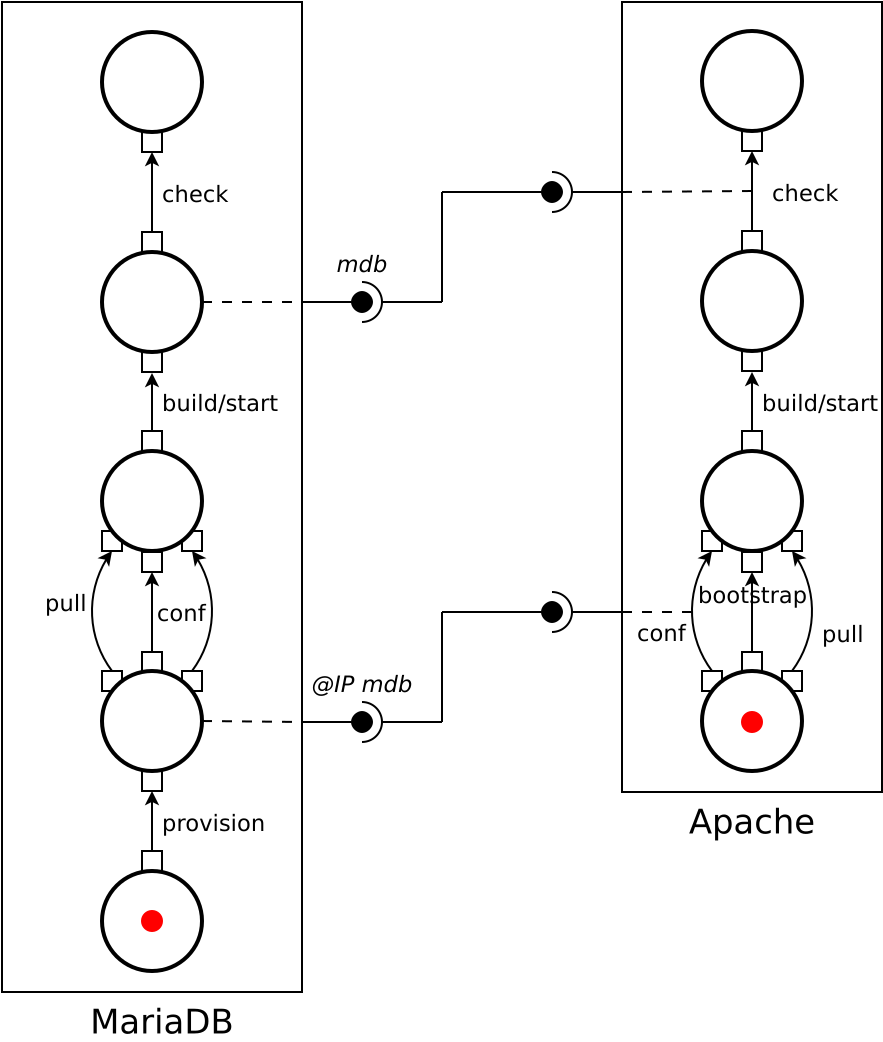
\includegraphics[width=0.7\linewidth]{./images/apachebdd.pdf}
  \end{center}
  \caption{Example of a commissioning assembly with two components
    Apache and MariaDB. Places are represented by circles, transitions
    by arrows between places, service ports by small black circles and
    semi-circles, data ports by outgoing or incoming arrows from
    components. Two initial red tokens are placed in each initial
    place of components in this example.}
  \label{fig:example}
\end{figure}

\paragraph{Example}{ Figure~\ref{fig:example} depicts the Madeus
  commissioning of an Apache web server and a MariaDB database. This
  example is based on a real container-based deployment described by
  RedHat\footnote{\url{https://access.redhat.com/documentation/en-us/red_hat_enterprise_linux_atomic_host/7/html/getting_started_with_containers/install_and_deploy_an_apache_web_server_container}}%
  $^,$%
  \footnote{\url{https://access.redhat.com/documentation/en-us/red_hat_enterprise_linux_atomic_host/7/html/getting_started_with_containers/install_and_deploy_a_mariadb_container}}. Two
  component types are declared by using Madeus is this example: Apache
  and MariaDB. Apache contains four places, or millestones, while
  MariaDB contains five places. Some parallel transitions are declared
  for each of the component and can be observed in the figure. Both
  components have two ports. MariaDB provides both a data and a
  service (once installed), while Apache uses a service and a
  data. Figure~\ref{fig:example} shows the assembly of one Apache and
  one MariaDB instanciated from their component types. These instances
  are connected by their ports. Indeed, the Apache configuration need
  the IP adress of the MariaDB component, and the testing phase for
  Apache, called \texttt{check}, uses the MariaDB service.}

In Madeus two kind of \emph{actors} are considered. First, the
developer of a control component, called \emph{dev-comp}, who may be
the same developer as the associated existing piece of code, or
another developer, or even a system operator or administrator. Second,
the developer of an assembly, called \emph{dev-ass}, who is typically
\HC[All]{le nom me fait rire :D} a system operator or administrator
who wants to write the overall commissioning procedure of a
distributed software system to deploy on its infrastructure. One
important difference bewteen Madeus and other approaches is its clear
separation of concerns between the commissioning of a single component
and the composition of an assembly, without taking care of the
detailed commissioning of each component. Even if Ansible, Puppet and
Chef, for instance, offer properties close to composition (\eg roles,
playbooks, recipes etc.), the system operator still have to handle the
correct order of composition. Conversely, the correct coordination,
thus the correct order of execution, is automatically guaranteed by
Madeus by the composition of the component instances. The composition
view point is illustrated in Figure~\ref{fig:simple} where
\emph{dev-ass} does not need to know the details of each component to
compose them. Such property has also been offered by Aeolus~\cite{}
but without parallelism within components.

\begin{figure}[tbp]
  \begin{center}
    \includegraphics[width=0.6\linewidth]{./images/simpleass.pdf}
  \end{center}
  \caption{Madeus assembly of an Apache component and a MariaDB
    component without knowing the details of each component.}
  \label{fig:simple}
\end{figure}

Madeus is a language to model distributed software commissionings,
thus Madeus is a \emph{meta-model}. Second, Madeus is a
\emph{graphical language}, as illustrated in Figure~\ref{fig:example},
that can be used to observe and understand how a distributed software
commissioning is modeled, but also to be able to monitor the state of
this procedure. Third, Madeus also comes with a \emph{concrete
  language}, which is for now prototyped in Python. Finally, Madeus is
able to execute one assembly by following a formal \emph{operational
  semantics}. In this sub-section we give an overview of the
meta-model, the concrete language and the execution semantics of
Madeus by using the example of Figure~\ref{fig:example}. Later
Sections~\ref{sec:forma_model} and~\ref{sec:perf_model} will present
the formalization of Madeus and its operational semantics, as well as
its theoretical performance model.

%%%%%%%%%%%%%%%%%%%%%%%%%%
\subsection{Meta-model}

\HC[Maverick]{figures a refaire avec nos discussions}

\begin{figure}[tbp]
  \begin{center}
    \includegraphics[width=0.9\linewidth]{./images/ass_uml.pdf}
  \end{center}
  \caption{Madeus meta-model of an assembly, \ie an overall
    commissioning procedure of a distributed software.}
  \label{fig:mmass}
\end{figure}

Figures~\ref{fig:mmass} and~\ref{fig:mmcomp} respectively depict the
UML diagram representing the Madeus meta-model of an assembly, and the
meta-model of a component. A Madeus assembly is not different from a
usual assembly in any component model of the literature. An assembly
basically contains component instances, connected between each other
through their compatible ports. One specificity is that Madeus handles
four types of ports instead of usually two, by dissociating service
ports from data ports which have different semantics. Intuitively,
unlike service ports, data ports act as data registries thus, once
activated, they will never be disabled.

\begin{figure}[tbp]
  \begin{center}
    \includegraphics[width=0.9\linewidth]{./images/component_uml.pdf}
  \end{center}
  \caption{Madeus meta-model of a component, \ie the commissioning
    procedure of a single component (\ie module or service).}
  \label{fig:mmcomp}
\end{figure}

However, as already explained a Madeus component is very different
from usual components in the literature. A component type contains a
set of places, a set of transitions, and a set of service-provide,
service-use, data-rpovide and data-user ports.
%Each place contains
%input and output docks. A transition is composed of a source and a
%destination dock (from one place to another). Docks are used in the
%formal model to properly handle parallelism and
%synchronizations.
Service-provide ports (service or data) are bound to groups of
places. Those groups of places represent the sub-part of the
commissioning procedures where a given service is provided. A
data-provide port is simply bound to one place from which the data is
provided. Use ports (data or service) are bound to transitions where
the corresponding data or services modeled by ports are actually used
by the transition function.

%%%%%%%%%%%%%%%%%%%%%%%%%%
\subsection{Concrete language}

\HC[Maverick]{syntaxe a discuter en fonction de la petite surcouhe
  faite a concerto}

The concrete syntax of Madeus has been implemented in Python. Madeus
is a simple declarative language that follows the meta-model
previously detailed to define, first, component types, and second,
assemblies of components. Listing~\ref{codemdb} shows the declaration
of the MariaDB component type of Figure~\ref{fig:example}. Lines 3 to
8 consist in the declaration of the places of the component type. A
place is identified by a unique \texttt{string}. Lines 9 to 15 consist
in the declaration of the transitions of the component type. A
transition is identified by a unique key (a \texttt{string}), and is
associated through a dictionnary to a source and a destination
place. Moreover, each transition is associated to a function to call
to perform associated actions. For instance, the function
\texttt{f\_pull} of transition \texttt{pull} is declared line 20 and
will contain the code to execute during this transition. Finally lines
16 to 19 declare the ports of the component type. A port is identified
by a unique key (a \texttt{string}), and is associated to a type and
the elements to which it is bound. As already described,
service-provide ports are bound to a set of places, data-provide ports
to a single place, and both service-use and data-use ports to a set of
transitions. In the case of MariaDB one service-provide port, namely
\texttt{serv}, is provided both at \texttt{std} and \texttt{chd}
places, and one data-rpovide port, namely \texttt{ip} is provided from
the first place \texttt{wtg}.

\begin{lstlisting}[label=codemdb,caption=Madeus code of the MariaDB
  component type.]
class MariaDB (MadeusComponent):
  def create(self):
    self.places = [
        'wtg',
        'prd',
        'cfd',
        'std',
        'chd'
    ]
    self.initial_place = 'wtg'
    self.transitions = {
        'provision': ('wtg','prd', self.f_prov),
        'pull': ('prd', 'cfd', self.f_pull),
        'conf': ('prd', 'cfd', self.f_conf),
        'bootstrap': ('prd', 'cfd', self.f_boots),
        'start': ('cfd', 'std', self.f_start),
        'check': ('std', 'chd', self.f_check)
    }
    self.dependencies = {
        'ip': (DepType.DATA_PROVIDE, 'wtg'),
        'serv': (DepType.PROVIDE, ['std','chd'])
    }
    
    def f_prov(self):
        # execution of bash scripts
        # execution of ansible playbooks
        # etc.
    def f_pull(self):
        # ...
    def f_conf(self):
        # ...
    def f_boots(self):
        # ...
    def f_start(self):
        # ...
    def f_check(self):
        # ...
\end{lstlisting}


Similarly, the Listing~\ref{codeapache} shows the decalaration of the
Apache component type of Figure~\ref{fig:example} which has one place
and one transition more than MariaDB. Furthermore, the Apache
component type contains one service-use port and one data-use port
(lines 18 to 21).

\begin{lstlisting}[label=codeapache,caption=Madeus code of the Apache
  component type.]
class Apache (MadeusComponent):
  def create(self):
    self.places = [
        'wtg',
        'cfd',
        'std',
        'chd'
    ]
    self.initial_place = 'wtg'
    self.transitions = {
        'pull': ('wtg', 'cfd', self.f_pull),
        'conf': ('wtg', 'cfd', self.f_conf),
        'bootstrap': ('wtg', 'cfd', self.f_boots),
        'start': ('cfd', 'std', self.f_start),
        'check': ('std', 'chd', self.f_check)
    }
    self.dependencies = {
        'ipMDB': (DepType.DATA_USE, ['conf']),
        'serviceMDB': (DepType.USE, ['check'])
    }

    def f_pull(self):
        # execution of bash scripts
        # execution of ansible playbooks
        # etc.
    def f_conf(self):
        # ...
    def f_boots(self):
        # ...
    def f_start(self):
        # ...
    def f_check(self):
        # ...
\end{lstlisting}


Finally, the Listing~\ref{codeass} shows the decalaration of the
assembly of components of Figure~\ref{fig:example}. First, lines 6 and
7 respectively instanciate component types MariaDB and Apache
previously declared. Second, line 9 to 13 are as follows: the creation
of an assembly, the addition of component instances to the assembly,
the connections of the components. Finally, lines 15 and 16 run the
assembly to perform the commissioning of MariaDB/Apache. An overview
of this execution is given in the next section.

\begin{lstlisting}[label=codeass,caption=Madeus code of the assembly
  of Figure~\ref{fig:example}.]
from components.mariadb import MariaDB
from components.apache import Apache

class ApacheWithDB (MadeusAssembly):
  def create():
    self.components = {
      'apache': Apache(),
      'mariadb': MariaDB()
    }
    self.dependencies = [
      ('apache', 'ipMDB', 'mariadb', 'ip'),
      ('apache', 'servMDB', 'mariadb', 'serv')
    ]

if __name__ == '__main__':
  assembly = ApacheWithDB()
  assembly.run()
\end{lstlisting}


%%%%%%%%%%%%%%%%%%%%%%%%%%
\subsection{Execution}

In \mad, executing a commissioning procedure requires to execute an
assembly. \HC[Helene, Maverick]{TODO introduire la notion de token}
The \mad execution model is governed by operational semantics rules to
move tokens from places to transitions within components. Those rules
are inspired from Petri nets rules but Madeus places and transitions
are different from Petri nets places and transitions, and additional
elements such as groups or ports also makes Madeus different from
Petri nets. Details of the transformation from a Madeus assembly to a
Petri net has been given in~\cite{}. \mad is executed by seven
operational semantics rules. In this section we only sketch the role
of each of these rules that will be formally given in
Section~\ref{sec:forma_model}. Before giving the role of each rule,
one can note in Figure~\ref{fig:example} the small rectangles that
have not been explained yet. These rectangles are \emph{docks}. Each
place has input and output transitions, and each transition has a
source dock and a destination dock. Docks have not been detailed
previously because they are automatically infered from the concrete
syntax of Madeus. Though, this concept is needed to explain the
execution of a Madeus assembly as it is used to handle parallelism and
synchronization of transitions.
%
\begin{enumerate}
\item \emph{Firing a transition}: when the source dock of a transition
  contains a token and when all use ports of a transition have their
  associated connections activated, the token is moved from the source
  dock to the transition, which is not considered atomic as it is
  associated to an action function.
\item \emph{Ending a transition}: when a transition holds a token and
  when the action associated to the transition is terminated, the
  token is moved from the transition to its destination dock.
\item \emph{Joining a place}: when all input docks associated to a
  place hold a token, tokens can be merged to a single one placed
  within the place.
\item \emph{Leaving a place}: when a place holds a token, and if all
  provide ports hold by this place are not used by other components,
  the token can be duplicated and placed in each output dock of the
  place.
\item \emph{Enabling use-provide connection}: a use-provide connection
  which is disabled can be enabled when the place associated to the
  provide port holds a token.
\item \emph{Disabling use-provide connection}: a use-provide
  connection which is enabled becomes disabled when a token leaves the
  place associated to the provide port.
\item \emph{Enabling data connection}: a data-use-provide connection
  which is disabled can be enabled when the place associated to the
  provide port holds a token. In this case the value is taken from one
  of the previous transition actions.
\end{enumerate}

One can note that a data connection cannot be disabled. It
indefinitely holds the last data value.
%\CP[HC]{Correct?}
%\HC{je n'ai pas parlé des groupes pour simplifier le discours. je ne pense pas en parler car ce n'est pas utile dans les exemples.}
%\CP{ok}

\begin{figure}[tbp]
  \begin{center}
    \includegraphics[width=0.7\linewidth]{./images/scenari.pdf}
  \end{center}
  \caption{Three deployment scenarios of the deployment, represented by three colors.}
  \label{fig:scenari}
\end{figure}

\subsubsection*{Apache/MariaDB Example: \mad Execution}

We discuss now the deployment execution for the Apache/MariaDB
example.  The initial assembly, given in Figure~\ref{fig:example}, has
already been described. Figure~\ref{fig:scenari} depicts three example
scenarios that may happen at different steps of the deployment, the
first one with red tokens, the second one with blue tokens, and the
third one with green tokens.

First, one can note that as MariaDB provides its IP address in its
first place, the associated connection between MariaDB and Apache is
immediately enabled. In the first scenario, the red token of MariaDB
has been able to move from its initial place to its three output
docks. Then, each transition in each branch is able to start as they
are not bound to any port. Simultaneously, the Apache component has
been able to start its \emph{provision} transition and reaches its
parallel branches: \emph{pull} and \emph{conf} can directly start. The
\emph{conf} transition, however, has to wait its associated connection
to be enabled. As the connection has been enabled in the first place
of MariaDB, the red token of the source dock of \emph{conf} can move
to \emph{conf}.

In the second scenario (blue tokens), the MariaDB component has reached
its second place. Both \emph{bootstrap} and \emph{conf} transitions of Apache
have finished but the \emph{pull} transition is still running. For this
reasons the three docks responsible for the join will not release the
tokens until \emph{pull} is terminated. As soon as \emph{pull}
finishes, the three tokens are merged into one token and set to the
next place.%, as MariaDB has already publishes an IP on the data port.

The third scenario illustrates an example where MariaDB reaches
its last place. As soon as this place holds a token, its associated
provide connection is enabled. Reversely, the \emph{check}
transition of Apache that is using services of MariaDB is able to
start, once the connection is enabled.

%-------------------------------------------------------
\section{The formal model}
\label{sec:forma_model}
%-------------------------------------------------------
%--------------------------
\subsection{Component}
%--------------------------

Formally in \mad, a component is defined as a tuple that can be divided
into four different parts: \emph{places}, \emph{transitions}, \emph{ports} and
\emph{bindings}.

\paragraph{Places}{

A component in \mad is first defined by a set of \emph{places} denoted
$\Pi$. A component is also defined by two sets of
\emph{docks}. A dock is represented by a small square and is attached to a
place. It is used to handle synchronization of parallel branches. The
first set concerns input docks. It is denoted $\Delta_{i}$ and it is
displayed under the place they are attached to. The second set is
denoted $\Delta_{o}$. It contains output docks and is displayed above
the place they are attached to.
The function $place\,:\,\Delta_{o}\cup\Delta_{i}\rightarrow\Pi$
returns the place a dock is attached to. Functions
$dock_i\,:\,\Pi\rightarrow \mathcal{P}(\Delta_{i})$ and
$dock_o\,:\,\Pi\rightarrow \mathcal{P}(\Delta_{o})$ respectively
returns the subset of $\Delta_i$ and $\Delta_o$ attached to a place
$\pi\in\Pi$. Places can be part of one or multiple groups which are
subsets of $\Pi$. The set of groups is denoted $G$. Last, $I \subseteq \Pi$ is the
non-empty set of initial places of the component.

}

\paragraph{Transitions}{

  % -----
\begin{table}[tp]
  \centering
  \resizebox{\columnwidth}{!}{%
    \begin{tabular}{|c|c|}
      \hline
      & \emph{Places}\\
      \hline
      $\Pi$ & set of places of a component\\
      $\Delta_{i}$ & set of input docks of a component\\
      $\Delta_{o}$ & set of output docks of a component\\
      $place$ & function mapping a dock to its place\\
      $dock_{i}$ & function mapping a place to its input docks\\
      $dock_{o}$ & function mapping a place to its output docks\\
      $G$ & set of groups of places\\
      $I$ & subset of places holding a token at initialization\\
      \hline
      \hline
      & \emph{Transitions}\\
      \hline
      $\Theta$ & finite set of transitions\\
      $A$ & finite set of actions\\
      $action$ & function mapping a transition to its corresponding action\\
      $end$ & function indicating if the action of the transition has finished\\
      \hline
      \hline
      & \emph{Ports}\\
      \hline
      $P_{u}$ & set of use ports of a component\\
      $P_{p}$ & set of provide ports\\
      $T_{port}$ & set of types of ports\\
      $type_{p}$ & function mapping a port to its type\\
      $D_{u}$ & set of data use ports of a component\\
      $D_{p}$ & set of data provide ports\\
      $T_{data}$ & set of types of data ports\\
      $type_{d}$ & function mapping a data port to its type\\
      $\mathbb{D}$ & set of possible data values\\
      \hline
      \hline
      & \emph{Bindings}\\
      \hline
      $B_{P_{u}}$ & set of pairs mapping use ports to transitions\\
      $B_{P_{p}}$ & set of pairs mapping provide ports to groups of places\\
      $B_{D_{u}}$ & set of pairs mapping data use ports to transitions\\
      $B_{D_{p}}$ & set of pairs mapping data provide ports to places\\
      \hline
      \hline
      & \emph{Assembly}\\
      \hline
      $C$ & set of component instances of an assembly\\
      $L_{P}$ & set of use-provide connections of an assembly\\
      $L_{D}$ & set of data-use-provide connections of an assembly\\
      $ebl$ & function indicating if a connection is enabled\\
      \hline
      \hline
      & \emph{Semantics}\\
      \hline
      $mk$ & function indicating if an element holds a token\\
      $val_{A,D_p}$ & returns the value given by an action to a data-provide port\\
      $val$ & function mapping a data provide port to its current value\\
      \hline
    \end{tabular}
  }
  \caption{Notations used throughout this paper}
  \label{tab:not}
\end{table}
%-----
A component is also defined by a set of \emph{transitions} denoted
$\Theta$. A transition $\theta \in \Theta$ is a pair containing one
source dock and one destination dock: $\theta =
\left(s,d\right)\,:\,s\in\Delta_{o},\,d\in\Delta_{i}$. 
%\CP{d=i $=>$ i is not defined! $d\in\Delta_i$ tout simplement, non ?}.
%
Each transition is associated to an \emph{action}. The set of actions is
denoted $A$ and the function $action\,:\,\Theta\rightarrow A$ gives the action
associated to a given transition. Finally, the function
$end\,:\,A\rightarrow\mathbb{B}$, where $\mathbb{B}=\left\{
\text{true},\text{false}\right\}$ indicates whether the action of a
transition has finished.
  
}

\paragraph{Ports}{

Places and transitions are internal elements of a \mad component.
The external interfaces of a component in \mad is
composed of \emph{ports}. A component contains a set of \emph{use-ports}
denoted $P_{u}$, and a set of \emph{provide-ports}, denoted
$P_{p}$. Each port is associated to a type in $T_{port}$, and the
function $type_{p}\,:\,P_{u}\cup P_{p}\rightarrow T_{port}$ maps the ports
to their type. 

In addition to traditional use-provide ports of component models,
\mad handles a specific use-provide abstraction for the
transfer of data values. These ports are called \emph{data-use-ports}
and \emph{data-provide-ports}. The set of data-use ports is denoted
$D_{u}$, and the set of data-provide ports is denoted
$D_{p}$. The set of possible data values is denoted
by $\mathbb{D}$. Finally, the function $type_{d}\,:\,D_{u}\cup
D_{p}\rightarrow T_{data}$ returns the data type of a given data port. In
  
}

\paragraph{Bindings}{

In a \mad component, places, groups of places and transitions can be
bound to ports through \emph{bindings}. There are four sets of bindings.
First, we denote $B_{P_{u}}$ the set of pairs that maps
each use port to one or multiple internal transitions in $\Theta$, indicating
that these transitions use the service associated to this port: 
$\left(p,\theta\right)\,:\,p\in P_{u},\,\theta\in\Theta$. Second, we
denote $B_{P_{p}}$ the set of pairs that maps each provide port to one or
multiple groups of places, indicating that if at least one token exists in each
group, the port is active: $\left(p,g\right)\,:\,p\in
P_{p},\,g\in G$. Third, we denote $B_{D_{u}}$ the set of pairs that
maps each data use port to one or multiple internal transitions in $\Theta$,
indicating that these transitions use the data associated to this port: 
$\left(d,\theta\right)\,:\,d\in D_{u},\,\theta\in\Theta$. Finally, we
denote $B_{D_{p}}$ the set of pairs that maps each data provide port to
one or multiple places, indicating that the data associated to this port is
available if a token is or has been in one of these places: $\left(d,\pi\right)\,:\,d\in
D_{p},\,\pi\in \Pi$. 
}

%--------------------------
\subsection{Assembly}
%--------------------------

An \emph{assembly} of components represents the instantiation of
components as defined in the previous section, and their connections
through their ports. In \mad an assembly is defined as a triplet
$(C, L_{P}, L_{D})$, where $C$ is a finite set of component instances,
$L_{P}$ is the set of connections (links) between use ports and
provide ports of compatible types, and $L_{D}$ is the set of
connections between data-use ports and data-provide ports of
compatible types. For all the components $c_1,\dots,c_n \in C$, we
denote with a star any union of the corresponding sets, for instance
$\Pi^* = \Pi_1 \cup \dots \cup \Pi_n$. We give a similar definition
for functions, for instance
$type_{p}^*\,:\,P_{u}^*\cup P_{p}^*\rightarrow T_{port}$. Connections
are defined as follows:

\begin{itemize}
\item $\left(u,p\right)\ \in L_{P},:\,u\in P_{u}^{*},\,p\in P_{p}^{*},\,type_{p}^{*}\left(u\right)=type_{p}^{*}\left(p\right)$,
\item $\left(u,p\right)\ \in L_{D},:\,u\in D_{u}^{*},\,p\in D_{p}^{*},\,type_{d}^{*}\left(u\right)=type_{d}^{*}\left(p\right)$.
\end{itemize}

%--------------------------
\subsection{Operational semantics}
%--------------------------

At each moment in the execution of a \mad deployment assembly
$(C, L_{P}, L_{D})$, we define three functions giving the current
status of this assembly. First, we denote the function
$ebl\,:\,L_{P}\cup L_{D}\rightarrow\mathbb{B}$, where
$\mathbb{B}=\left\{ \text{true},\text{false}\right\}$, that indicates
if a connection is enabled or not. This \emph{enabling} concept on
connections will be used to coordinate component deployments. Second,
the marking function is defined to evaluate if one element of any
component holds a token:
$mk\,:\,\Pi^{*}\cup\Delta_{i}^{*}\cup\Delta_{o}^{*}\cup\Theta^{*}\rightarrow\mathbb{B}$
where $\mathbb{B}=\left\{ \text{true},\text{false}\right\}$. By
construction, an element can either hold one or zero tokens, the
formal proof of this being left as future work.

Third, we define the function
$val\,:\,D_{P}^{*}\rightarrow \mathbb{D}\cup\left\{ \text{null}\right\}$
that returns the current value associated to a data provide port.

We call a \emph{valuation} the tuple $\left\langle mk,ebl,val\right\rangle$,
where $mk$ indicates where tokens are located, $ebl$ indicates whether
connections are enabled or not, and $val$ indicates the current value
of any data provide port.
At initialization the valuation is defined as follows:
\begin{itemize}
\item $mk\left(x\right)=\begin{cases}
\text{true} & \text{if }x\in I^{*}\\
\text{false} & \text{if } x\in\left(\Pi^{*}\setminus I^*\right)\cup\Delta_{i}^{*}\cup\Delta_{o}^{*}\cup\Theta^{*}
\end{cases}$
\item $ebl\left(l\right)=\text{false}\quad\forall l \in L_{P}\cup L_{D}$
\item $val\left(d\right)=\text{null}\quad\forall d \in D^*_{p}$
\end{itemize}

\noindent\textbf{Notations.}
\begin{itemize}
  \item For a function $f\,:\,A\rightarrow B$, we denote $f^{\prime}=f\left[a\coloneqq b\right]\,:\,A\rightarrow B$ such that:
    \begin{equation*}
      f^{\prime}\left(x\right)=\begin{cases}
      b & \text{if }x=a\\
      f\left(x\right) & \text{if }x\neq a
      \end{cases}.
    \end{equation*}
  \item We define the function $val_{A,D_p}\,:\,A\times
    D_{P}^*\rightarrow \mathbb{D}$ that returns the data value to assign to a
    given data-provide port after an action.
\end{itemize}
    
In this paper, we present seven rules to operate the \mad model. We
leave for future work the extension of these rules to support errors
and reconfigurations. The rules are formally defined in
Figure \ref{fig:rules}.

\paragraph{Firing transition}{

The first rule of \mad is formally defined by
Equation~(\ref{eq:r1}). The upper part of the rule indicates the
hypotheses needed to fire a transition, \ie starting a transition,
and the lower part indicates the conclusion of the rule, \ie the valuation
changes. To fire a transition, the source dock of the transition
$\theta$ needs a token, and for any port bound to the transition
$\theta$ the connection of this port must be enabled. The conclusion of
this rule is to move the token from the output dock to the
transition. The upper part of Figure~\ref{fig:r1} illustrates the
hypotheses and the lower part the conclusion of the rule.

\begin{figure}[t]
\begin{center}
  \includegraphics[width=0.55\columnwidth]{./images/firing.pdf}
\end{center}
\caption{Illustration of the rule of Equation~(\ref{eq:r1}) to fire transitions.}
\label{fig:r1}
\end{figure}

}

\paragraph{Ending transition}{

The second rule of \mad is formally defined by
Equation~(\ref{eq:r2}). To end a transition $\theta$, a token has to
be present on the transition and the action performed by the
transition must be terminated. When ending a transition, the token
is moved from this transition to its destination dock. Note that the ports bound
to the transition cannot be disconnected before applying this rule. Moreover, if
the place to which the destination dock is attached is bound to
data-provide ports, their values are replaced by those computed by the action.
For this reason, the rule uses the function
$val_{A,D_p}$. Figure~\ref{fig:r2} illustrates this rule.
%\MC{Expliquer pourquoi les ports ne peuvent pas etre deconnectes ?}

\begin{figure}[t]
\begin{center}
  \includegraphics[width=0.55\columnwidth]{./images/ending_transition.pdf}
\end{center}
\caption{Illustration of the rule of Equation~(\ref{eq:r2}) to end transitions.}
\label{fig:r2}
\end{figure}
  
}

\paragraph{Input docks to place}{

The third rule of \mad is formally defined by
Equation~(\ref{eq:r3}). To move tokens from input docks of a place to
this place, all input docks must hold a token. The conclusion is to remove
all the tokens within the docks and to add one token inside the
place as illustrated in Figure~\ref{fig:r3}.

\begin{figure}[t]

\begin{minipage}[h]{0.45\columnwidth}%
  \centering
  \includegraphics[width=0.65\columnwidth]{./images/inputdocks_to_place.pdf}
  \captionof{figure}{\label{fig:r3}Illustration of the rule of Equation~(\ref{eq:r3}) to move tokens from input docks to a place.}
\end{minipage}
\hfill
\begin{minipage}[h]{0.45\columnwidth}%
  \centering
  \includegraphics[width=0.65\columnwidth]{./images/place_to_outputdocks.pdf}
  \captionof{figure}{\label{fig:r4}Illustration of the rule of Equation~(\ref{eq:r4}) to move tokens from place to output docks.}
\end{minipage}
\end{figure}

\paragraph{Place to output docks}{

The fourth rule of \mad is formally defined by
Equation~(\ref{eq:r4}). To move a token from a place to its output
docks, a token needs to be present onto the place. Also, if the place
is part of a group which is itself bound to a used provide port,
applying the rule must not make the last token of the group leave,
otherwise this provide port becomes inactive. A provide port is said
to be used if it is connected to a use port bound to a transition
holding a token.  If these conditions are met, the token can be
removed from the place, and a token is added onto each output dock
attached to this place. This rule is illustrated in
Figure~\ref{fig:r4} in a simplified manner.

}

\paragraph{Enabling use-provide connections}{

The fifth rule of \mad is formally defined by
Equation~(\ref{eq:r5}). To enable a connection between use and provide
ports, at least one token has to be present in each group of places
bound to the provide port. A token is considered present in a group if
it is placed on one of the places, or on a transition between docks,
one of these docks being attached to one place of the group. The
conclusion of the rule is the enabling of the connection as depicted
in Figure~\ref{fig:r5}.

\begin{figure}[t]
  \begin{center}
    \includegraphics[width=0.7\columnwidth]{./images/link_service.pdf}

    \caption{Illustration of the rule of Equation~(\ref{eq:r5}) to enable a
    connection between use and provide ports of an assembly.}

    \label{fig:r5}
  \end{center}
\end{figure}
  
}

\paragraph{Disabling use-provide connections}{

The sixth rule of \mad is formally defined by
Equation~(\ref{eq:r6}). Note that this rule has maximum priority and
must be executed first if applicable. To disable a connection between
use and provide ports, there must not be any token in any group of
places bound to the provide port. The conclusion of the rule is to disable
the connection as depicted in Figure~\ref{fig:r6}.

\begin{figure}[t]
\begin{center}
  \includegraphics[width=0.7\columnwidth]{./images/break_service.pdf}
\end{center}
\caption{Illustration of the rule of Equation~(\ref{eq:r6}) to disable a connection between use and provide ports of an assembly.}
\label{fig:r6}
\end{figure}

}

\paragraph{Enabling data-use-provide connections}{

Finally, the seventh rule of \mad is formally defined by
Equation~(\ref{eq:r7}). To enable a connection between data-use and
data-provide ports, a value has to be associated to the data-provide
port. The conclusion of the rule is the activation of the connection as
depicted in Figure~\ref{fig:r7}. One can note that the position of
tokens is not a hypothesis in this rule. Actually, we consider in
the formal model that once a value has been attached to a data-provide
port, by applying the rule that ends a transition
(Equation~(\ref{eq:r2})), the connection of this port can be enabled
and will never be disabled. In pratice though, a disabling rule for
data ports could be usefull to not consume extra resources.
  
\begin{figure}[t]
\begin{center}
  \includegraphics[width=0.4\columnwidth]{./images/link_data.pdf}
\end{center}
\caption{Illustration of the rule of Equation~(\ref{eq:r7}) to enable a connection between data-use and data-provide ports of an assembly.}
\label{fig:r7}
\end{figure}

}

%------------
\begin{figure*}[tp]
%
\begin{equation}
\cfrac{\theta =\left(s,d\right) \in \Theta^*,s \in \Delta_o^*,d \in \Delta_i^*\qquad mk\left(s\right)\qquad\forall p \in P_{u}\cup D_{u},\left(p,\theta\right)\in B_{P_{u}}^{*}\cup B_{D_{U}}^{*}\,:\,\text{is\_ready}(p)}{\left\langle mk,ebl,val\right\rangle \rightarrow\left\langle mk\left[s\coloneqq\text{false}\right]\left[\theta\coloneqq\text{true}\right],ebl,val\right\rangle }
\label{eq:r1}
\end{equation}
%
\begin{equation*}
  \text{where: }\text{is\_ready}(p) = \exists\left(a,b\right)\in L_{S}\cup L_{D},\,a=p\land ebl\left(a,b\right).
\end{equation*}
%
\begin{equation}
\cfrac{\theta=\left(s,d\right) \in \Theta^*\qquad mk\left(\theta\right)\qquad end\left(action\left(\theta\right)\right)}{\left\langle mk,ebl,val\right\rangle \rightarrow\left\langle mk\left[\theta\coloneqq\text{false}\right]\left[d\coloneqq\text{true}\right],ebl,val\left[\forall p\in D_P^*,\text{dest}(p)\,:\, p\coloneqq val_{A,D_p}(action(\theta),p)\right]\right\rangle}
\label{eq:r2}
\end{equation}
%
\begin{equation*}
  \text{where: }\text{dest}(p) = \left(p,g\right)\in B_{D_{p}}^*,place(d)\in g
\end{equation*}
%
\begin{equation}
\cfrac{\pi\in\Pi^*\qquad D_i=dock_i(\pi)\qquad\forall\delta\in D_i\,mk\left(\delta\right)}{\left\langle mk,ebl,val\right\rangle \rightarrow\left\langle mk\left[\forall\delta\in D_i\,:\,\delta\coloneqq\text{false}\right]\left[\pi\coloneqq\text{true}\right],ebl,val\right\rangle }
\label{eq:r3}
\end{equation}
%
\begin{equation}
\cfrac{\pi\in\Pi^{*}\qquad D_o=dock_o(\pi)\qquad mk\left(\pi\right)\qquad \forall g\in G,\pi\in g:\,\text{can\_leave}\left(\pi,D_o,g\right)}{\left\langle mk,ebl,val\right\rangle \rightarrow\left\langle mk\left[\forall\delta\in D_o\,:\,\delta\coloneqq\text{true}\right]\left[\pi\coloneqq\text{false}\right],ebl,val\right\rangle }
\label{eq:r4}
\end{equation}
%
\begin{align*}
\text{where: }\text{can\_leave}\left(\pi,D_o,g\right) = & \left(\exists p,(p,g)\in B_{P_p}:\,\text{is\_used}(p)\right)\implies \lnot \text{last\_token\_leaves} \left(\pi,D_o,g\right) \\
\text{is\_used}\left(p\right) = & \exists u\in P_{u}^{*},\theta\in\Theta^{*}:~\left(p,u\right)\in L_{P}\land \left(u,\theta\right)\in B_{P_u}^{*}\land mk\left(\theta\right) \\
\text{last\_token\_leaves}\left(\pi,D_o,g\right) = & \left(\text{is\_group\_enabled}\left(g,mk\right)\land\lnot \text{is\_group\_enabled} \left(g,mk\left[\pi\coloneqq \text{false}\right]\left[\forall d\in D_o \,:\,d\coloneqq \text{true}\right]\right)\right) \\
\text{is\_group\_enabled}\left(g,mk\right) = & \left(\exists\,\pi\in g:\,mk\left(\pi\right)\right)\\
 & \, \lor\left(\exists\,\delta\in\Delta_{o}^{*}\cup\Delta_{i}^{*}:\,mk\left(\delta\right)\land \left(\exists(s,d)\in\Theta^{*}:\,\left(\delta=s\lor \delta=d\right)\land \text{is\_in\_group}\left((s,d),g\right)\right)\right)\\
 & \, \lor\left(\exists\,\theta\in\Theta^{*}:\,mk\left(\theta\right)\land \text{is\_in\_group}\left(\theta,g\right)\right) \\
\text{is\_in\_group}\left((s,d),g\right) = & place\left(s\right)\in g\land place\left(d\right)\in g
\end{align*}
%
\begin{equation}
\cfrac{l = (u,p)\in L_{S}\qquad\lnot ebl\left(l\right)\qquad\forall g \in G,\left(p,g\right)\in B_{P_{p}}\,:\,\text{is\_group\_enabled}\left(g,mk\right)}{\left\langle mk,ebl,val\right\rangle \rightarrow\left\langle mk,ebl\left[l\coloneqq\text{true}\right],val\right\rangle }
\label{eq:r5}
\end{equation}
%
\begin{equation}
\cfrac{l=(u,p)\in L_{S}\qquad ebl\left(l\right)\qquad\exists g \in G,\left(p,g\right)\in B_{P_{p}}\,:\,\lnot\text{is\_group\_enabled}\left(g,mk\right)}{\left\langle mk,ebl,val\right\rangle \rightarrow\left\langle mk,ebl\left[l\coloneqq\text{false}\right],val\right\rangle }
\label{eq:r6}
\end{equation}
%
\begin{equation}
\cfrac{l=(u,p)\in L_{D}\qquad\lnot ebl\left(l\right)\qquad val\left(p\right)\neq\text{null}}{\left\langle mk,ebl,val\right\rangle \rightarrow\left\langle mk,ebl\left[l\coloneqq\text{true}\right],val\right\rangle }
\label{eq:r7}
\end{equation}
%
\caption{The seven operational semantics rules of \mad.}
\label{fig:rules}
\end{figure*}
%------------

%--------------------------
%\subsection{Consistency rule}
%--------------------------
\textbf{Consistency.}

In \mad, the maximum number of tokens that can be used is the number
of possible parallel branches. A token can only be created during a
branching (rule \emph{place to output docks}), where one token is
created for each output dock of the place. For this reason, cycles are
forbidden in \mad, otherwise an infinity of tokens could be created
which does not make sense within a deployment. We plan in future work
on reconfiguration to allow cycles in very specific settings to keep
control on the tokens and their creation.

\HC[All]{Maybe the performance model in this section too if short
  enough}

%-------------------------------------------------------
\section{The performance model}
\label{sec:perf_model}
%-------------------------------------------------------
In this section, we present a theoretical performance prediction model
for \mad that estimates the total execution time of the
commissionning of a given assembly, according to the execution time of
each transition. Three goals are pursued with such a tool. First, the
theoretical execution time offers a way to evaluate the quality of the
prototype of \mad. Second, for a system administrator or a developer,
knowing the theoretical execution time of the commissioning procedure
is useful. Third, in the case of a fully autonomic commissioning and
reconfiguration process, which is left to future work, theoretical
information on the execution time is needed to take adequate
decisions, in particular for critical systems and services.

To build this performance prediction model, we need an estimation of
the execution time of all the actions in the assembly, given as a
function $time\,:\,\actions\rightarrow\mathbb{R}^+$.  Computing
precise execution times for the kind of actions used in a deployment
can be difficult and is itself the subject of many studies, \eg using
an analytical model or a statistical approach. However, for our
application, we find that estimates are sufficient as long as they preserve
the relative difference between different transitions.
%
Intuitively, we automatically deduce the execution flow of a \mad
assembly based on \mad' formal semantics. This is done by generating a
dependency graph representing the execution flow of each \mad
component in the assembly and connecting them together according to their
dependencies (the connections between their ports). Then, a
\emph{source} vertex is connected to the vertices representing the beginning of
the execution of each component, and a \emph{sink} vertex is connected to
the vertices representing the end of the execution of each component.
%
Thus, a dependency graph representing the execution of the whole
assembly is obtained. By weighting the arcs corresponding to the transitions with
the individual execution times of their actions (and the other ones with 0),
we can compute the expected total execution time of the assembly as the
longest path from the \emph{source} vertex to the \emph{sink} vertex.

% By generating a graph modelling the execution flow of a \mad assembly,
% capturing both intra-component and inter-component dependencies, we
% reduce this problem to finding the longest path in a DAG.

\subsection{Assumptions}

The performance model given here is valid only for assemblies such
that any set of places bound to a provide port contains exactly one
place. If a provide port is bound to a set containing multiple
places, the requirement imposed by this binding is satisfied as soon
as one of the places is reached. The total time then depends on the
earliest time at which one of these places is reached, which cannot be
modeled as a longest path. In practice this is not a severe
restriction, as ports requirements very rarely include
disjunctions. Indeed, none of our use-cases relies on this
feature. However, we still consider the possibility of having multiple
sets (of one place) bound to a port. In this case, the port is enabled
when all the places are reached.

%% \MC{Préciser ici que dans la pratique ce n'est pas un problème ?}
%% \HC[Maverick et Simon]{oui, j'ai commencé une phrase, il faut donner
%%   l'intuition du problème posé par la disjonction et aussi dire que
%%   dans la pratique sur des cas réels nous n'avons jamais eu besoin de
%%   disjonctions.}

The estimation provided by the model is a best case scenario: it
assumes that all actions are started as soon as possible, and that the
hardware has the capacity to run all possible parallel actions without
affecting their execution times.

%--------------------------------------
\subsection{Notations}
%--------------------------------------

%% Recall that given a component, we denote its set of places $\Pi$ and its
%% set of transitions $\Theta$. In the following, we consider that the
%% transitions go directly from a place to
%% another place instead of from an output dock to an input dock.
%% Hence, $\Theta$ is a multiset which elements are pairs of places.
%% \MC[Maverick,Simon]{Si on change les transitions pour qu'elles contiennent l'action,
%% plus besoin de parler de multiset je pense (+TODO ce ne sont plus des paires)}
%We
%can obtain the place corresponding to each dock by using the $place$
%function of the component.

%% We also consider the following two functions:
%% \begin{itemize}
%% \item the \emph{group entrance function} $g_{in}\,:\,G\rightarrow\mathcal{P}\left(\Pi\right)$ with\\
%% $g_{in}(g)=\left\{ \pi\,\mid\,\pi\in g\land\exists\pi_{b}\,:\,\left(\pi_{b}\not\in g\land\left(\pi_{b},\pi\right)\in\Theta\right)\right\} $
%% (the result of $g_{in}$ is called the set of \emph{entrance places}
%% of the group)
%% \item the \emph{group exit function} $g_{out}\,:\,G\rightarrow\mathcal{P}\left(\Pi\right)$ with\\
%% $g_{out}(g)=\left\{ \pi\,\mid\,\pi\in g\land\exists\pi_{a}\,:\,\left(\pi_{a}\not\in g\land\left(\pi,\pi_{a}\right)\in\Theta\right)\right\} $
%% (the result of $g_{out}$ is called the set of \emph{exit places}
%% of the group)
%% \end{itemize}

Recall that an assembly is a tuple $A = (C,L)$. In the following, for
any component $c_i \in C$, any of its associated set is denoted
$X_i$, \eg $\Pi_i$ for the set of places of the component $c_i$.  As
previously, for each set $X$ defining a component, we denote $X^*$ the
union (in the case of an assembly) or the extension (in the case of a
function) for all components. For instance
$\Pi^*=\bigcup_{i=1}^{n}\Pi_i$ denotes the set of all places in the
assembly.

The execution flow graph is an oriented weighted graph $\left(V,E\right)$
where $V$ is the set of vertices and $E$ is the set of weighted
arcs with elements in $V\times \mathbb{R}^{+} \times V$. We define
$V$ and $E$ in the following.

%--------------------------------------
\subsection{Vertices}
%--------------------------------------

For each place, we introduce two vertices: one representing the place
itself and one representing the event of a token leaving the place.
\[
V_{\Pi}=\bigcup_{\pi\in\Pi^*}\left\{ v_\pi^\text{place},v_\pi^\text{leav}\right\} 
\]
\MC[Maverick]{TODO : vérifier si on peut fusionner les deux sommets de
  place}
\HC[Maverick]{si c'est long a verifier, laisser comme ça, il faut
  qu'on soumette !}

For each transition, we introduce two vertices: one representing the
beginning of the transition and one representing its end.
\[
V_{\Theta}=\bigcup_{\theta\in\Theta^*}\left\{ v_\theta^\text{beg},v_\theta^\text{end}\right\} 
\]

\SR{On peut sans doute retirer les vertices representant les ports, et
  directement connecter $v^{place}_\pi$ à $v^{beg}_\theta$.}
\HC[Maverick et Simon]{oui je pense aussi, mais même remarque que au
  dessus, il faut qu'on soumette !}
For each provide port we introduce one vertex representing its enabling.
\[
V_{S_p}=\bigcup_{p\in S_p^*} \left\{ v_p^\text{start}\right\} 
\]


Finally, we define $V$ as the union of all these, plus one source
and one sink vertices. 
\[
V=V_{\Pi}\cup V_{\Theta} \cup V_{S_p} \cup \left\{ v^\text{source},v^\text{sink}\right\} 
\]

%--------------------------------------
\subsection{Arcs}
%--------------------------------------

In the dependency graph, arcs represent time constraints: the event represented
by the destination vertex must happen after the one represented by the source
vertex, at least $w$ seconds apart where $w$ is the weight of the arc. In
practice, arcs corresponding to actions are weighed with the corresponding
time, while other arcs have a weight 0 and merely represent a dependency.

For each place $\pi$ we introduce one arc from $v_\pi^\text{place}$ to
$v_\pi^\text{leav}$. This represents the fact that a token may leave $\pi$
only after it has entered it.
Figure~\ref{fig:place_graph} depicts the dependency graph corresponding to a place.
\[
E_{\Pi}=\bigcup_{\pi\in\Pi^*}\left\{ \left(v_\pi^\text{place},0,v_\pi^\text{leav}\right)\right\} 
\]

%%%%%%%%%%%%%%%
\begin{figure}[h]
  \subfloat[\mad place]{%
    \fcolorbox{black!20}{white}{
      \begin{minipage}[c][2.5cm][c]{0.43\linewidth}%
        \centering
        \includegraphics[scale=0.15]{images/perf_place.pdf}
      \end{minipage}
    }
  }
  \subfloat[Dependency graph]{%
    \fcolorbox{black!20}{white}{
      \begin{minipage}[c[c][2.5cm][c]{0.43\linewidth}%
        \centering
        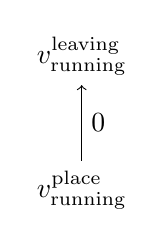
\begin{tikzpicture}[node distance=1.7cm]
          \node (leaving) [] {$v_\text{running}^\text{leaving}$};
          \node (place) [below of=leaving] {$v_\text{running}^\text{place}$};
          \draw [->] (place) -- (leaving) node[midway, right] {$0$};
        \end{tikzpicture}
      \end{minipage}
    }
  }
  \caption{Part of the dependency graph generated from a \mad place}
  \label{fig:place_graph}
\end{figure}

For each transition $\theta = (s, \alpha, d)$, we introduce
three arcs. The first between $v_\theta^\text{beg}$ and $v_\theta^\text{end}$
represents the fact that the end of $\theta$ happens at the time of the
start of $\theta$ plus the time required for the action $\alpha$. The second between $v_{\pi(s)}^\text{leav}$
and $v_\theta^\text{beg}$ represents the fact that $\theta$ may only
happen after a token has left $\pi(s)$. The third one between $v_\theta^\text{end}$ and
$v_{\pi(d)}^\text{place}$ represents the fact that a token may enter $\pi(d)$ only
after $\theta$ has ended.
Figure~\ref{fig:transition_graph} depicts the dependency graph corresponding to three
transitions \emph{t1}, \emph{t2} and \emph{t3}.
\begin{align*}
E_{\Theta}=\bigcup_{\theta=(s,\alpha,d)\in\Theta^*} & \left\{ \left(v_\theta^\text{beg},time(\alpha),v_\theta^\text{end}\right),\right.\\
 & \left(v_{\pi(s)}^\text{leav},0,v_\theta^\text{beg}\right),\left. \left(v_\theta^\text{end},0,v_{\pi(d)}^\text{place}\right)\right\}
\end{align*}

%%%%%%%%%%%%%%%
\begin{figure}[h]
  \subfloat[\mad internal net example]{
    \fcolorbox{black!20}{white}{
      \begin{minipage}[c][4cm][c]{0.33\linewidth}%
        \centering
        \includegraphics[width=0.8\columnwidth]{images/perf_transition.pdf} \label{fig:transmadeus}
      \end{minipage}
    }
  }
  \subfloat[Dependency graph]{
    \fcolorbox{black!20}{white}{
      \begin{minipage}[c][4cm][c]{0.53\linewidth}%
        \centering
        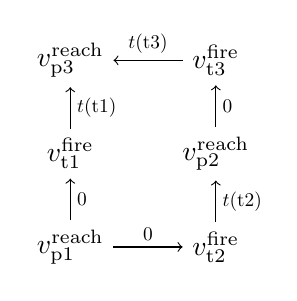
\begin{tikzpicture}[node distance=1.7cm]
          \node (p3) [] {$v_\text{p3}^\text{reach}$};
          \node (t1) [below =15pt of p3] {$v_\text{t1}^\text{fire}$};
          \node (p1) [below =15pt of t1] {$v_\text{p1}^\text{reach}$};
          \node (t2) [right =25pt of p1] {$v_\text{t2}^\text{fire}$};
          \node (p2) [above =15pt of t2] {$v_\text{p2}^\text{reach}$};
          \node (t3) [above =15pt of p2] {$v_\text{t3}^\text{fire}$};
          \draw [->] (t3) -- (p3) node[midway, above, scale=0.7] {$t(\text{t3})$};
          \draw [->] (t2) -- (p2) node[midway, right, scale=0.7] {$t(\text{t2})$};
          \draw [->] (t1) -- (p3) node[midway, right, scale=0.7] {$t(\text{t1})$};
          \draw [->] (p1) -- (t1) node[midway, right, scale=0.7] {$0$};
          \draw [->] (p1) -- (t2) node[midway, above, scale=0.7] {$0$};
          \draw [->] (p2) -- (t3) node[midway, right, scale=0.7] {$0$};
        \end{tikzpicture}
        \label{fig:transdag}
      \end{minipage}
    }
  }
  \caption{A set of \mad transitions and their corresponding equivalent dependency graph}
  \label{fig:transition_graph}
\end{figure}


%% SR: text before modification
%% For each data-provide port $p$, we associate (a) for each binding between
%% $p$ and a place $\pi$ one arc from $v_\pi^\text{place}$ to
%% $v_p^\text{start}$, and (b) for each connection connecting $p$
%% to a data-use port $u$, for each binding between $u$ and a transition
%% $\theta$ one arc from $v_p^\text{start}$ to $v_\theta^\text{beg}$.

For each data-provide port $p$ and each place $\pi$ such that
$\{\pi\}$ is bound to $p$, we introduce one arc from
$v_\pi^\text{place}$ to $v_p^\text{start}$. This represents the
enabling of the port after all (set of) places bound to the port
have been reached.
\[
A_{S_p}= \bigcup_{(p,\{\pi\})\in B_{S_p}^*}\left\{ \left(v_\pi^\text{place},0,v_p^\text{start}\right)\right\}
\]

Additionally, for each provide port $p$ and each transition
$\theta$ such that $p$ is connected to a use port that is bound
to $\theta$, we introduce one arc from $v_p^\text{start}$ to
$v_\theta^\text{beg}$. This represents the activation of the transitions
bound to a use port, after the port is provided.
\[
E_{S_u} = \bigcup_{\substack{(u,p)\in L \\ (u,\theta)\in B_{S_u}^*}} \left\{ \left(v_p^\text{start},0,v_\theta^\text{beg}\right)\right\}
\]

Figure~\ref{fig:ports_graph} depicts the dependency graph corresponding to a
provide port \emph{p} bound to a place \emph{c1p} and connected to
a use port \emph{u} which is bound to a transition \emph{c2t}.
\SR[Maverick]{TODO: change figure (part a)}

%% SR: text before modification
%% Figure~\ref{fig:data_ports_graph} depicts the dependency graph corresponding to a
%% data-provide port \emph{dp} bound to a place \emph{c1p} and connected to
%% a data-use port \emph{du} which is bound to a transition \emph{c2t}.
%% \begin{align*}
%% A_{D}=\bigcup_{p\in D_p}
%% & \left(\bigcup_{\pi,\,\left(p,\pi\right)\in B_{D_{p}}^*}\left\{ \left(v_\pi^\text{place},v_p^\text{start},0\right)\right\}\right. \\
%% & \left.\cup\bigcup_{\substack{u,\,\left(u,p\right)\in L_D \\
%%   \theta,\,\left(u,\theta\right)\in B_{D_{u}}^*}}\left\{ \left(v_p^\text{start},v_\theta^\text{beg},0\right)\right\}\right)
%% \end{align*}

%%%%%%%%%%%%%%%
\begin{figure}[h]
  \subfloat[\mad port connection]{%
    \fcolorbox{black!20}{white}{
      \begin{minipage}[c][2cm][c]{0.34\linewidth}%
        \centering
        \includegraphics[scale=0.14]{images/perf_data_ports.pdf}
        \label{fig:port}
      \end{minipage}
    }
  }
  \subfloat[Dependency graph]{%
    \fcolorbox{black!20}{white}{
      \begin{minipage}[c][2cm][c]{0.52\linewidth}%
        \centering
        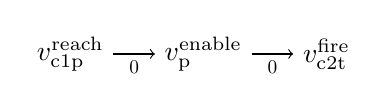
\begin{tikzpicture}[node distance=1.7cm]
          \node (c1p1) [] {$v_\text{c1p}^\text{reach}$};
          \node (p) [right =15pt of c1p1] {$v_\text{p}^\text{enable}$};
          \node (c2t) [right =15pt of p] {$v_\text{c2t}^\text{fire}$};
          \draw [->] (c1p1) -- (p) node[midway, below, scale=0.7] {$0$};
          \draw [->] (p) -- (c2t) node[midway, below, scale=0.7] {$0$};
        \end{tikzpicture}
        \label{fig:portdag}
      \end{minipage}
    }
  }
  \caption{A connection and its corresponding dependency graph}
  \label{fig:ports_graph}
\end{figure}


%% SR: text before modification (see below) 
%% For each service-provide port $p$, we associate (a) for each binding between
%% $p$ and a group $g$ one arc from $v_\pi^\text{place}$ to $v_p^\text{start}$
%% for each $\pi$ in $g_{in}(g)$ and one arc from $v_p^\text{stop}$ to
%% $v_\pi^\text{leav}$ for each place $\pi$ $g_{out}(g)$, and (b) for each
%% connection connecting $p$ to a service-use port $u$, for each binding between
%% $u$ and a transition $\theta$ one arc from $v_p^\text{start}$ to
%% $v_\theta^\text{beg}$ and one arc from $v_\theta^\text{end}$ to
%% $v_p^\text{stop}$.
%% The (a) arcs represent the fact that the service becomes available when all
%% groups bound to it have a token, and each of them can be deactivated only when
%% the provide port is not used anymore. The (b) arcs represent the
%% fact that the transitions bound to a service-use port may only execute once
%% the port is provided, and do not use the port anymore once they are over.

%% For each service-provide port $p$, each groupd $g$ bound to $p$ and
%% each place $\pi$ in $g_{in}(g)$, we introduce one arc from
%% $v_\pi^\text{place}$ to $v_p^\text{start}$, representing the
%% availability of the service once all groups bound to it hold a token.

%% Conversely, for each each service-provide port $p$, each group $g$
%% bound to $p$ and each place $\pi$ in $g_{out}(g)$, we introduce one
%% arc from $v_p^\text{stop}$ to $v_\pi^\text{leav}$, in order to
%% represent the fact that the group $g$ may not be disabled while the
%% port is busy.

%% Lastly, for each service-provide port $p$ and each transition $\theta$
%% such that $p$ is connected to a service-use port bound to $\theta$, we
%% introduce one arc from $v_p^\text{start}$ to $v_\theta^\text{beg}$ and
%% one arc from $v_\theta^\text{end}$ to $v_p^\text{stop}$. They
%% represent the activation of the transitions bound to a service-use
%% port after it has been provided, and the release of the port after the
%% transition is over.

%% Figure~\ref{fig:service_ports_graph} depicts the dependency graph corresponding to a
%% service-provide port \emph{sp} bound to a group with \emph{c1p1} as entrance
%% place and \emph{c1p2} as exit place, and connected to service-use port
%% \emph{su} which is bound to transition \emph{c2t}.

%% \begin{alignat*}{3}
%% A_{S}=\bigcup_{p\in S_p}
%% & \left(\bigcup_{g,\,\left(p,g\right)\in B_{S_{p}}^*} \right. && \left. \left(\bigcup_{\pi\in g_{in}(g)} \left\{\left(v_\pi^\text{place},v_p^\text{start},0\right)\right\}\right.\right. \\
%% &&& \left. \cup\left.\bigcup_{\pi\in g_{out}(g)} \left\{\left(v_p^\text{stop},v_\pi^\text{leav},0\right)\right\}\right)\right. \\
%% & \left.\cup\bigcup_{\substack{u,\,\left(u,p\right)\in L_S \\
%%       \theta,\,\left(u,\theta\right)\in B_{S_{u}}^*}} \right. && \left. \left\{ \left(v_p^\text{start},v_\theta^\text{beg},0\right),\right.\right. \left.\left.\left(v_\theta^\text{end},v_p^\text{stop},0\right)\right.\Big\}\right.\Bigg)
%% \end{alignat*}

%%%%%%%%%%%%%%%
%%\begin{figure}[t]
  \subfloat[\mad use-provide connection]{%
    \fcolorbox{black!20}{white}{
      \begin{minipage}[c]{0.95\columnwidth}%
        \centering
        \includegraphics[scale=0.15]{images/perf_service_ports.pdf}
      \end{minipage}
    }
  }
  \\

  \subfloat[Dependency graph]{%
    \fcolorbox{black!20}{white}{
      \begin{minipage}[c]{0.95\columnwidth}%
        \centering
        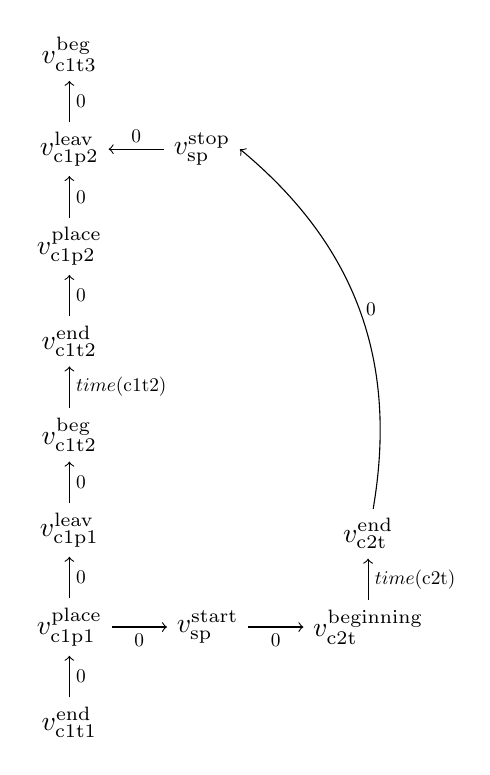
\begin{tikzpicture}[node distance=1.7cm]
          \node (c1t3) [] {$v_\text{c1t3}^\text{beg}$};
          \node (c1p2l) [below =15pt of c1t3] {$v_\text{c1p2}^\text{leav}$};
          \node (c1p2) [below =15pt of c1p2l] {$v_\text{c1p2}^\text{place}$};
          \node (c1t2_end) [below =15pt of c1p2] {$v_\text{c1t2}^\text{end}$};
          \node (c1t2) [below =15pt of c1t2_end] {$v_\text{c1t2}^\text{beg}$};
          \node (c1p1l) [below =15pt of c1t2] {$v_\text{c1p1}^\text{leav}$};
          \node (c1p1) [below =15pt of c1p1l] {$v_\text{c1p1}^\text{place}$};
          \node (c1t1_end) [below =15pt of c1p1] {$v_\text{c1t1}^\text{end}$};
          \draw [->] (c1t1_end) -- (c1p1) node[midway, right, scale=0.7] {$0$};
          \draw [->] (c1p1) -- (c1p1l) node[midway, right, scale=0.7] {$0$};
          \draw [->] (c1p1l) -- (c1t2) node[midway, right, scale=0.7] {$0$};
          \draw [->] (c1t2) -- (c1t2_end) node[midway, right, scale=0.7] {$time(\text{c1t2})$};
          \draw [->] (c1t2_end) -- (c1p2) node[midway, right, scale=0.7] {$0$};
          \draw [->] (c1p2) -- (c1p2l) node[midway, right, scale=0.7] {$0$};
          \draw [->] (c1p2l) -- (c1t3) node[midway, right, scale=0.7] {$0$};
          \node (sp) [right =20pt of c1p1] {$v_\text{sp}^\text{start}$};
          \node (c2t) [right =20pt of sp] {$v_\text{c2t}^\text{beginning}$};
          \node (c2t_end) [above =15pt of c2t] {$v_\text{c2t}^\text{end}$};
          \node (sps) [right =20pt of c1p2l] {$v_\text{sp}^\text{stop}$};
          \draw [->] (c2t) -- (c2t_end) node[midway, right, scale=0.7] {$time(\text{c2t})$};
          \draw [->] (c1p1) -- (sp) node[midway, below, scale=0.7] {$0$};
          \draw [->] (sp) -- (c2t) node[midway, below, scale=0.7] {$0$};
          \draw [->] (c2t_end) to[bend right] node[midway, right, scale=0.7] {$0$}(sps.east) ;
          \draw [->] (sps) -- (c1p2l) node[midway, above, scale=0.7] {$0$};
        \end{tikzpicture}
      \end{minipage}
    }
  }
  \caption{Vertices and arcs for service ports, bindings and connections}
  \label{fig:service_ports_graph}
\end{figure}

For each initial place $\pi$ we introduce one arc from $v^\text{source}$
to $v_\pi^\text{place}$, representing the fact that a token is placed in each
initial place in the initial configuration.
Figure~\ref{fig:source_sink_graph} depicts the dependency graph corresponding to two initial
places \emph{c1p1} and \emph{c2p2}.
\[
E_I=\bigcup_{\pi, \Delta_i(\pi) = \emptyset}\left\{ \left(v^\text{source},0,v_\pi^\text{place}\right)\right\} 
\]

For each final place $\pi$ we introduce one arc from $v_\pi^\text{place}$
to $v^\text{sink}$. Intuitively, this represents the fact that the
commissionning is over only after all components have reached the
places without outgoing transitions.
Figure~\ref{fig:source_sink_graph} depicts the dependency graph
corresponding to three final places \emph{c1p2}, \emph{c2p2}
and \emph{c2p3}.
\[
E_F=\bigcup_{\pi, \Delta_o(\pi) = \emptyset}\left\{ \left(v_\pi^\text{place},0,v^\text{sink}\right)\right\} 
\]

%%%%%%%%%%%%%%%
\begin{figure}[t]
  \subfloat[\mad assembly]{%
    \begin{minipage}[c]{0.95\columnwidth}%
      \centering
      \includegraphics[scale=0.15]{images/perf_source_sink.pdf}
    \end{minipage}
  }
  \\
  
  \subfloat[Dependency graph]{%
    \fcolorbox{black!20}{white}{
      \begin{minipage}[c]{0.95\columnwidth}%
        \centering
        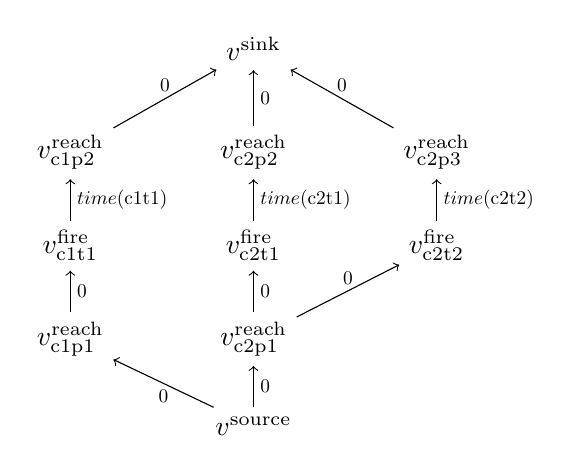
\begin{tikzpicture}[node distance=1.7cm]
          \node (c1p2) [] {$v_\text{c1p2}^\text{reach}$};
          \node (c1t1) [below =15pt of c1p2] {$v_\text{c1t1}^\text{fire}$};
          \node (c1p1) [below =15pt of c1t1] {$v_\text{c1p1}^\text{reach}$};
          \node (c2p2) [right =35pt of c1p2] {$v_\text{c2p2}^\text{reach}$};
          \node (c2t1) [below =15pt of c2p2] {$v_\text{c2t1}^\text{fire}$};
          \node (c2p1) [below =15pt of c2t1] {$v_\text{c2p1}^\text{reach}$};
          
          \node (c2p3) [right =35pt of c2p2] {$v_\text{c2p3}^\text{reach}$};
          \node (c2t2) [below =15pt of c2p3] {$v_\text{c2t2}^\text{fire}$};
          
          \node (source) [below =15pt of c2p1] {$v^\text{source}$};
          \node (sink) [above =20pt of c2p2] {$v^\text{sink}$};
          
          \draw [->] (c1t1) -> (c1p2) node[midway, right, scale=0.7] {$time(\text{c1t1})$};
          \draw [->] (c2t1) -- (c2p2) node[midway, right, scale=0.7] {$time(\text{c2t1})$};
          \draw [->] (c2t2) -- (c2p3) node[midway, right, scale=0.7] {$time(\text{c2t2})$};
          \draw [->] (c1p1) -- (c1t1) node[midway, right, scale=0.7] {$0$};
          \draw [->] (c2p1) -- (c2t1) node[midway, right, scale=0.7] {$0$};
          \draw [->] (c2p1) -- (c2t2) node[midway, above, scale=0.7] {$0$};
          \draw [->] (source) -- (c1p1) node[midway, below, scale=0.7]{$0$};
          \draw [->] (source) -- (c2p1) node[midway, right, scale=0.7] {$0$};
          \draw [->] (c1p2) -- (sink) node[midway, above, scale=0.7] {$0$};
          \draw [->] (c2p2) -- (sink) node[midway, right, scale=0.7] {$0$};
          \draw [->] (c2p3) -- (sink) node[midway, above, scale=0.7] {$0$};
        \end{tikzpicture}
      \end{minipage}
    }
  }
  \caption{Two components without ports and
    their equivalent dependency graph}
  \label{fig:source_sink_graph}
\end{figure}


Finally, we define $E$ as 
\[
E=E_\Pi\cup E_{\Theta} \cup E_{S_p}\cup E_{S_u}\cup E_{I}\cup E_{F}
\]

%--------------------------------------
\subsection{Time estimation}
%--------------------------------------

In the following, we denote $DG_A=(V,E)$ the dependency graph corresponding
to assembly $A=(C,L)$, and $DG_c$ the part of a dependency graph
corresponding to component $c \in C$.

We define the time estimation of the execution of the \mad assembly $A$
to be the length of a longest path between $v^\text{source}$ and
$v^\text{sink}$ in $DG_A$.

\begin{lemma}
 In $DG_A$, if $v^\text{sink}$ is reachable from $v^\text{source}$ and there
 are no cycles, then the time estimation for $A$ is well-defined.
 \label{lemma:well_defined}
\end{lemma}

\begin{proof}
 If $v^\text{sink}$ is reachable from $v^\text{source}$, there exists at least
 one path from $v^\text{source}$ to  $v^\text{sink}$. Because there are no
 cycles, the number of paths between $v^\text{source}$ and $v^\text{sink}$ is
 finite. Because all the paths have a weight, the set of longest paths is
 well-defined (and not empty). Therefore the length of a longest path is
 well-defined.
\end{proof}

\begin{lemma}
 In a component $c \in C$, if place $\pi_t \in \Pi$ is reachable from place
 $\pi_s \in \Pi$ (distinct from $\pi_t$), then $v_{\pi_t}^{place}$
 is reachable from $v_{\pi_s}^{place}$ in a $DG_c$.
 \label{lemma:reachable}
\end{lemma}

\begin{proof}
 Consider a path $P$ in the \net of $c \in C$ from $\pi_s$ to
 $\pi_t$ (this path exists because $\pi_t$ is reachable from
 $\pi_s$). This path is made of a sequence of places connected by
 transitions: $P=(\pi_s,t1,p2,t2,\dots,t_n,\pi_t)$.\\
 By construction, there exists a path\\
 $(v_{\pi_s}^{place},v_{\pi_s}^{leav},v_{t1}^{beg},v_{t1}^{end},v_{p2}^{place},\dots,v_{\pi_t}^{place})
 \in DG_c$.
\end{proof}


\begin{lemma}
 If an assembly $A$ has one or more components then $v^\text{sink}$ is
 reachable from $v^\text{source}$ in $DG_A$.
 \label{lemma:source_sink}
\end{lemma}

\begin{proof}
 Let us consider one component $c \in C$, its initial place $\pi_i$ and one of
 its final places $\pi_f$. By construction, $v_{\pi_i}^\text{place}$ is
 reachable from $v^\text{source}$, and $v^\text{sink}$ is reachable from
 $v_{\pi_f}^\text{place}$ in the dependency graph of an assembly containing this
 component. The last thing to prove is that $v_{\pi_f}^\text{place}$ is reachable
 from $v_{\pi_i}^\text{place}$ in $DG_c$.
 The end of the execution of a \mad component is defined as
 when all its tokens are in final places, \ie when there are no more
 transitions to perform. Therefore, by definition $\pi_f$ is
 necessarily reachable from $\pi_i$ in the \net of $c \in C$.
 We conclude by applying Lemma~\ref{lemma:reachable}.
\end{proof}

\begin{lemma}
 If a component $c \in C$ is well-formed then $DG_c$ has no cycle.
 \label{lemma:no_cycles_component}
\end{lemma}

\begin{proof}
 By construction, in $DG_c$ the vertices and arcs corresponding to places do
 not form cycles and are disjoint, so they cannot produce a cycle by themselves.
 Likewise, the arcs corresponding to port bindings have either their source
 vertex or their destination vertex of degree 1, so they cannot produce a cycle.
 Only the arcs corresponding to transitions can produce cycles. Moreover, the
 arcs in $DG_c$ connect only the vertices corresponding to the places which
 are connected in the \net. This means that if there is a cycle in $DG_c$,
 there is a cycle in the \net. However, the \net of a well-formed \mad component
 has no cycle. Therefore there are no cycles in $DG_c$.
\end{proof}

\begin{lemma}
 In an assembly $A$ of well-formed components with no deadlocks, if each port
 is bound to at most one element (place, transition or group) and if
 $\left|g_{in}(g)\right|\leq 1$ and $\left|g_{out}(g)\right|\leq 1$ for each group
 $g$ in $A$ then the $DG_A$ has no cycles.
 \label{lemma:no_cycles_assembly}
\end{lemma}

\begin{proof}
 By Lemma~\ref{lemma:no_cycles_component}, we have that the dependency graph
 of all the components in $A$ have no cycles.
 Then, the only way a cycle may exist in $DG_A$ is if the vertices and arcs
 corresponding to connections cause a cycle to exist.
 This may be acheived in two ways: because of a single service port bound to
 group $g$ if $\left|g_{out}(g)\right|>0$ (which implies by hypothesis
 $\left|g_{out}(g)\right|=1$); or because of two or more use and provide ports.
 First, because $\left|g_{out}(g)\right|=1$ (we consider $\pi_{out}$ to be the only
 place in $g_{out}(g)$), and because by construction $v_{\pi_{out}}^{leav}$ is
 reachable from $v_{\pi_{in}}^{place}$ (where $\pi_{in}$ is the only place in $g_{in}(g)$,
 then $v_{\pi_{in}}^{place}$ is not reachable from $v_{\pi_{out}}^{leav}$ (otherwise
 there would be a cycle in the dependency graph of the component). Second, a
 cycle can be caused by multiple connections if there are \emph{crossing
 dependencies} (see Figure~\ref{fig:deadlock}). However, this would create a
 deadlock in the assembly, which is not possible by hypothesis.
\end{proof}

\begin{figure}[t]
  \begin{center}
    \includegraphics[width=0.5\linewidth]{./images/deadlock.pdf}
  \end{center}
  \caption{Example of an invalid assembly: crossing dependencies cause a deadlock.}
  \label{fig:deadlock}
\end{figure}

\begin{theorem}
 In an assembly $A$ of one or more well-formed components with no deadlocks,
 if each port is bound to at most one element (place, transition or group) and if
 $\left|g_{in}(g)\right|\leq 1$ and $\left|g_{out}(g)\right|\leq 1$ for each group
 $g$ in $A$, then the time estimation obtained using $DG_A$ is well-defined.
 \label{theorem:well_defined}
\end{theorem}

\begin{proof}
 By applying Lemma~\ref{lemma:source_sink}, we know that $v^\text{sink}$ is reachable
 from $v^\text{source}$. By applying Lemma~\ref{lemma:no_cycles_assembly}, we know
 that there are no cycles in $DG_A$. We conclude by applying
 Lemma~\ref{lemma:well_defined}.
\end{proof}

\paragraph{Remark}

The restrictions imposed in \ref{theorem:well_defined} are here to consider only
assemblies for which the structure of the dependency graph does not change
depending on the duration of the transitions. To handle arbitrary assemblies,
a more complex performance model is needed, which is left as future work. In
practice, we expect most real-life assemblies to fulfill these requirements.
In particular, all of the assemblies presented in this article do.


\subsection{Complexity}

We now determine the size complexity of $DG_A=(V,E)$ and the time
complexity of computing the time estimation.

First, we notice that
$|V| \in \mathcal{O}\left(\left|\pi^*\right|+\left|\theta^*\right|+\left|S_{p^*}\right|+\left|D_{p^*}\right|\right)$
and
$|E| \in \mathcal{O}\left(\left|\pi^*\right|+\left|\theta^*\right|+\left|B_{S_p}\right|+\left|B_{D_p}\right|+\left|B_{S_u}\right|\times\left|L_S\right|\right.$ \\
$\left.+\left|B_{D_u}\right|\times\left|L_D\right|\right)$
.

Because $DG_A$ is a a directed acyclic graph, finding the longest path
between $v^\text{source}$ and $v^\text{sink}$, \ie finding a time estimation,
can be done in $\mathcal{O}(|V|+|E|)$ by sorting the
vertices topologically and iterating through them, computing their maximum
distance from the source using the one of their parents.



%-------------------------------------------------------
\section{Evaluations}
\label{sec:evaluations}
%-------------------------------------------------------
\HC[Maverick]{Il faudrait rappeler des détails sur l'implémentation du
prototype notamment sur la gestion du parallélisme en python}

Madeus is a model that relies on the description of a control
component for each software module of that will be deployed. It is a
low-level model, therefore the developer is responsible for the
choices of actions performed in the transitions.  This section
evaluates the performance of Madeus' prototype with empty transitions
in order to evaluate the \mad prototype independently of any specific
transitions. This is why these experiments are called
\emph{dry-runs}. It means the transitions do not contain any code or
command for which the execution time is unknown or imprecise, thus
allowing to measure the overhead caused by the prototype only. In
addition to this, the experiments presented in this section are
compared to the theoretical performance computed by the prediction
model detailed in Section~\ref{sec:perf_model}. By doing so we both
validate the theoretical performance model compared to the reality,
and the expected performance of the prototype on the set of use-cases.

\paragraph{Implementation details}
The prototype implementation was made in Python. Users declare components
by creating a class, inheriting from the \emph{Component} class, containing
the description of the \net as well as the actions associated to the
transitions. These actions are Python functions which usually perform remote
actions using SSH, Ansible or other tools. Users can then create an assembly
by extending the appropriate class and listing the components and how their
ports are connected. This assembly can then be run, which means that the
semantics of Madeus is executed in this assembly. The commissioning is
over if the only elements holding a token are places
without outgoing transitions. While this is not the case, the semantics is
executed by attempting to apply each rule from the semantics on each component.
When a transition is fired, the corresponding Python function is executed in
a Python thread, which does not block the execution of the semantics. Note
that Python threads do not take advantage of hardware parallelism capabilities,
but because the functions usually run other (possibly remote) processes to
do the heavy work, this is not an issue. The $\terminaction$ can be executed
for the corresponding function when it has finished its execution.

% figures to add for assemblies
%Sequential

\begin{figure}[h]
  \begin{center}
    \includegraphics[width=0.4\textwidth]{./images/seq.pdf}
    \caption{The \mad sequential assembly of Benchmark (A), with N components.}
    \label{fig:seq}
  \end{center}
\end{figure}

Three benchmarks compose this evaluation and are illustrated in
Figures~\ref{fig:seq} and~\ref{fig:par}.
% first
The first benchmark, denoted (A), models a sequential \mad assembly,
depicted in Figure~\ref{fig:seq}. It is composed of one
\emph{provider} component made of a transition and two places, and
$N+1$ \emph{user-provider} components that are also composed of a
transition and two places, but where the transition uses the provide
port of the preceeding component. The components are connected in
chain thus resulting in a sequential execution.
%The dry-run version of
%this assembly consists in transitions that do nothing besides wait for
%a fixed amount of time.
%The second version of this assembly features a transition that calls
%an ssh connection and waits for a fixed amount of time, similar as for
%the dry-run version, before finishing.

\begin{figure}[h]
  \begin{center}
    \includegraphics[width=0.4\textwidth]{./images/par.pdf}
    \caption{The \mad parallel assembly of Benchmark (B) and (C), with N parallel components, and T parallel transitions.}
    \label{fig:par}
  \end{center}
\end{figure}

%second
The two other benchmarks model \mad parallel assemblies and are
depicted in Figure~\ref{fig:par}. The first assembly, denoted (B)
evaluates the parallelism at the component level, called
\emph{inter-comp} and \emph{inter-comp-tasks} previously in this
paper. The second one, denoted (C), models the parallelism at the
transition level, \ie \emph{intra-comp-tasks}, when transitions are
performed simultaneously.
%
Both benchmarks use the same assembly that is composed of an initial
\emph{provider} component and $N$ parallel components connected to the
provider. Each component contains a first transition that uses the
service provided by the provider component and $T$ parallel
transitions. For Benchmark (B), the number of components varies from 1
to 40 components with a single transition per component $T=1$. For
Benchmark (C), the number of component is fixed to $N=1$ and the
number of transitions varies from 1 to 20.

Experiments have been performed on a single node of the \ecotype
cluster of the experimental platform
Grid'5000\footnote{\url{www.grid5000.fr}}. The detailed configuration
of the node is given in Table~\ref{tab:g5k}. Each experiment presented
in the results is an average of ten executions. For each transition
an execution time of 5 seconds has been applied. This execution time
is guaranteed by the call to the sleep function of \python. This
execution time has been chosen to get a coherent and readable scale of
results.
%They are both evaluated in \emph{dryrun} mode without any
%ssh connections and with \emph{ssh connections} active in the assembly
%between components, so as to allow visualisation of the eventual
%overhead of having these ssh connections.

\begin{figure}[h]
  \begin{center} 
    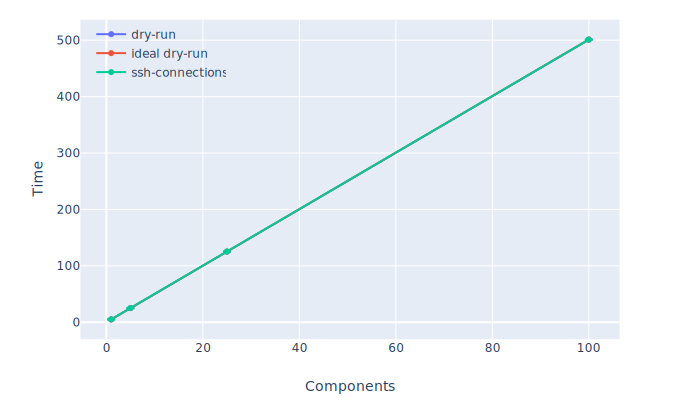
\includegraphics[width=0.5\textwidth]{./images/evaluations_sequential.pdf}
    \caption{Results of the sequential benchmark.}
    \label{fig:seqres}
  \end{center}
\end{figure}

Figure~\ref{fig:seqres} presents the results of Benchmark (A). As (A)
models a sequential assembly, the theoretical execution time is simply
the sum of the execution time of each transition of each component
($N+2$ components). The results show a linear increase in time and the
\emph{dryrun} curve follows the \emph{ideal} curve closely.
%The difference between the
%\emph{ssh-connections} curve is hard to visualise but is slightly
%higher than the \emph{ideal} and \emph{dryrun} curves, a logical
%result as the number of ssh connections grows with each component
%added, but there is always only one ssh connection at the same time.

\begin{figure}[h]
  \begin{center} 
    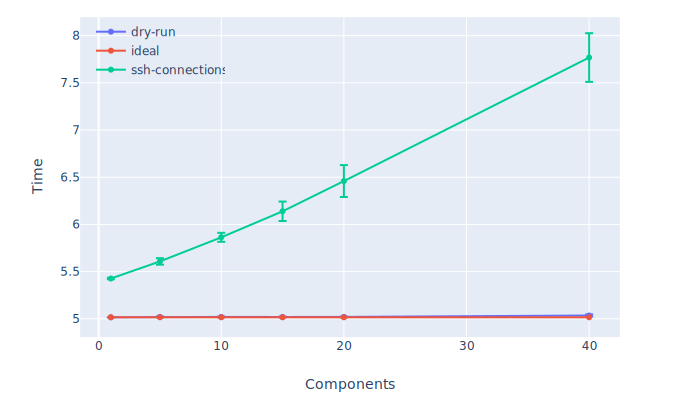
\includegraphics[width=0.5\textwidth]{./images/evaluations_par_component.pdf}
    \caption{Results of the parallel assembly benchmark with varying component number}
    \label{fig:parcompres}
  \end{center}
\end{figure}

% attention à comprendre si c'est systématique !
%For the results on the parallel assembly benchmark, we had to remove
%one outlier data point on the parallel assembly benchmark for
%component parallelism, as the first iteration of the assembly with
%just one component always had 4 seconds added to the time and we could
%not pinpoint the exact reason for that. As it did not occur for any of
%the other iterations, we did not take it into account on the curve
%drawing for our Figure~\ref{fig:parcompres}. In the results directory
%that can be found on our repository we have included the original
%times.json and the modified times.json files to keep the original
%results intact.

\HC[Charlène]{qu'est-ce qui a été exécuté exactement pour que ça soit
  5s le résultat ? ça ne colle pas à la figure de l'assemblage qui
  devrait donner 15s - faut-il refaire la figure ?}
Figure~\ref{fig:parcompres} depicts the results of Benchmark (B).  The
ideal theoretical performance for this benchmark is a constant equal
to the sleep duration time of transitions, \ie $5$ seconds. Indeed as
components are not connected together through ports they are deployed
simultaneously.
%value as components are commissioned in parallel. In \emph{dryrun}
%our experimental benchmark
One can note that the results observed with the \mad prototype is only
very slightly above the ideal constant result, which shows that the
prototype does not add significant overhead to the process even for a
large number of parallel components.
%The \emph{ssh connection} curve allows us to see
%that there is steady increase of time, adding almost 3 seconds to the
%assembly deployment when reaching 40 parallel components. This show
%that the overhead added by the SSH connections is not null.

\begin{figure}[h]
  \begin{center} 
    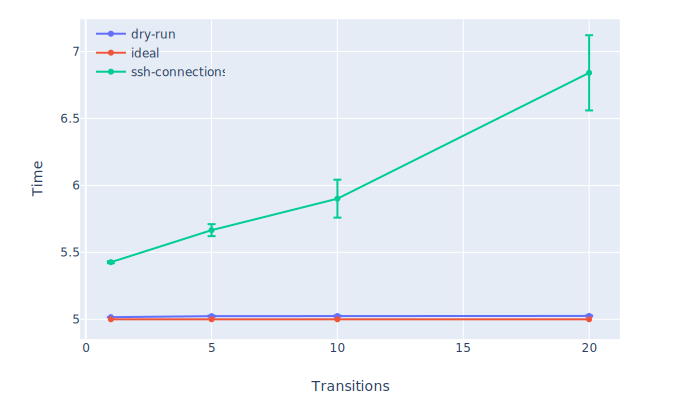
\includegraphics[width=0.5\textwidth]{./images/evaluations_par_transitions.pdf}
    \caption{Results of the parallel assembly benchmark with varying parallel transition number}
    \label{fig:partrans}
  \end{center}
\end{figure}

Figure~\ref{fig:partrans} shows the results for Benchmark (C). As for
the previous benchmark, and because transitions are executed
simultaneously in this benchmark, the theoretical expected curve is a
constant equal to the sleep duration time of transitions, \ie $5$
seconds. The results follow the ideal curve closely as well for a
large number of transitions.

%calculation for the ideal curve on the parallel assembly benchmark
%when varying the number of parallel transitions has been done in the
%same manner as for the parallel component variation. In \emph{dryrun}
%the benchmark results follow the ideal curve closely as well, whereas
%the \emph{ssh connections} curve has an overhead that grows as the
%number of transitions increases.

These results allow us to point out that \mad does not by itself add a
big overhead on the deployment. One can note though that according to
the type of commands performed in the transitions  an additional
overhead could be observed. For instance, .
\HC[Helene]{est-ce que c'est utile de donner l'exemple du surcoût SSH ?}
%They also show the
%importance of ssh connection and their impact on the deployment time.




%-------------------------------------------------------
\section{Conclusion}
\label{sec:conc}
%-------------------------------------------------------
\mad is a new component-based model specifically designed for distributed software commissioning procedures. By adapting composition mechanisms and combining them with the notion of control components, \mad enhances both the separation of concerns and the efficiency of commissioning compared to previous solutions. In this paper, the \mad model has been extensively presented from both the theoretical and experimental viewpoint.

First, after a detailed study of the related work, an overview of \mad
was given. Second, the formalization of \mad was presented, with a
streamlined theoretical model compared to our previous
publications. Third, a performance prediction model of \mad was
studied, based on the transformation of a \mad assembly into a
directed graph that represents the execution flow of the
assembly. Fourth, the prototype of \mad was evaluated on three
synthetic benchmarks and compared to the expected performance
predicted by the theoretical model. Results have shown that the
overhead introduced by the prototype is very low, and that the prediction
of the performance model is accurate. Finally, the benefits of \mad regarding
separation of concerns and efficiency have been evaluated and
discussed on a real complex use-case: the commissioning procedure of
OpenStack. Results have been extensively studied and have shown that
\mad outperforms both \ansible and \aeolus in terms of efficiency, and that a 
projection on the traces of the OpenStack CI could save 34 hours of computation a 
day.

As future work, first, \mad is currently not equipped with mechanisms to handle faults during the commissioning procedure. Notably, the rule $\terminaction$
does not consider the possibility of a failure during the action
$\alpha \in \exec$. We would like to equip \mad with if/else statements or switches as well as rollback mechanisms. Moreover, we would like to have formal guarantees in case of faults, for instance by using game theory or stochastic formal methods.

Second, we would like to study the semi-automatic (thanks to a very light DSL) or automatic (if possible) inference of dependencies from \ansible playbooks, so that \mad assemblies may be entirely or partially generated for the user.

Finally one can note that \mad has been generalized to dynamic reconfiguration of distributed software~\cite{ccgridmaverick}. Indeed, once commissioned, distributed software may need to adapt dynamically in order to respond to faults, to optimize some metrics (\eg energy, efficiency), or to adapt the services to dynamic requirements (\eg smart cities). When such reconfiguration decisions have to be taken, especially for critical systems, the duration of the reconfiguration should be taken into account. Thus, generalizing both \mad and the performance prediction models of Section~\ref{sec:perf_model} to dynamic reconfiguration is an important contribution.

  



%% \section*{Acknowledgment}

%% Experiments presented in this paper were carried out using the
%% Grid'5000 testbed, supported by a scientific interest group hosted by
%% Inria and including CNRS, RENATER and several Universities as well as
%% other organizations (see \url{https://www.grid5000.fr}).

% ---- Bibliography ----
\bibliographystyle{elsarticle-num-names}
% \bibliography{sigproc} 
\bibliography{main}

\end{document}
